% This is samplepaper.tex, a sample chapter demonstrating the
% LLNCS macro package for Springer Computer Science proceedings;
% Version 2.20 of 2017/10/04
%
\documentclass[runningheads]{llncs}
%
\usepackage{graphicx}
% Used for displaying a sample figure. If possible, figure files should
% be included in EPS format.

\usepackage[utf8]{inputenc}
\usepackage[english]{babel}
%\usepackage{amsthm}
\usepackage{amsmath}
\usepackage{amssymb}
\usepackage{float}
\usepackage{hyperref}
\usepackage{booktabs}
\usepackage{caption}
\usepackage{subcaption}
\usepackage[dvipsnames]{xcolor}
\usepackage{bm}
\usepackage[makeroom]{cancel}
\usepackage[inline]{enumitem}
\usepackage{cleveref}
\usepackage{placeins}

\usepackage[ruled,vlined]{algorithm2e}
%\newcommand\mycommfont[1]{\footnotesize\ttfamily\textcolor{blue}{#1}}
%\SetCommentSty{mycommfont}
\SetKwComment{Comment}{$\triangleright$\ }{}

\usepackage[%
square,        % for square brackets
comma,         % use commas as separators
%  numbers,       % for numerical citations;
%  sort,          % orders multiple citations into the sequence in which they appear in the list of references;
%sort&compress, % as sort but in addition multiple numerical citations
% are compressed if possible (as 3-6, 15);
]{natbib}
% In the bibliography, references have to be formatted as 1., 2., ... not [1], [2], ...
\renewcommand{\bibnumfmt}[1]{#1.}

\renewcommand{\bibsection}{\section*{References}} % requried for natbib to have "References" printed and as section*, not chapter*
% Use natbib compatbile splncsnat style.
% It does provide all features of splncs03, but is developed in a clean way.
% Source: http://phaseportrait.blogspot.de/2011/02/natbib-compatible-bibtex-style-bst-file.html
\bibliographystyle{splncsnat}

\usepackage{todonotes}
%\usepackage[disable]{todonotes}
\newcommand{\oam}[1]{\todo[inline,color=orange!40]{{\textbf{OM:}~}#1}}
\newcommand{\el}[1]{\todo[inline,color=green!40]{{\textbf{EL:}~}#1}}



%%%%%%%%%%%%%%%%%%%%%%%%%%%%
% Paper dependent stuff    %
%%%%%%%%%%%%%%%%%%%%%%%%%%%%

\newcommand{\Tau}{T}

\newcommand{\hlrb}[1]{\bm{\textcolor{Red}{#1}}}
\newcommand{\hlbb}[1]{\bm{\textcolor{Blue}{#1}}}
\newcommand{\hlgb}[1]{\bm{\textcolor{Green}{#1}}}

\newcommand{\OPD}{\texttt{OPD}}

%%%%%%%%%%%%%%%%%%%%%%%%%%%%
% Aesthetics               %
% over-underline, hat, bold%
%%%%%%%%%%%%%%%%%%%%%%%%%%%%

\newcommand{\eps}{\varepsilon}
\newcommand{\vareps}{\varepsilon}
\renewcommand{\epsilon}{\varepsilon}
%\renewcommand{\hat}{\widehat}
\renewcommand{\tilde}{\widetilde}
\renewcommand{\bar}{\overline}

\newcommand*{\MyDef}{\mathrm{\tiny def}}
\newcommand*{\eqdefU}{\ensuremath{\mathop{\overset{\MyDef}{=}}}}% Unscaled version
% \newcommand*{\eqdef}{\mathop{\overset{\MyDef}{\resizebox{\widthof{\eqdefU}}{\heightof{=}}{=}}}}
\newcommand{\eqdef}{\stackrel{def}{=}}


\def\:#1{\protect \ifmmode {\mathbf{#1}} \else {\textbf{#1}} \fi}
\newcommand{\CommaBin}{\mathbin{\raisebox{0.5ex}{,}}}

\newcommand{\wt}[1]{\widetilde{#1}}
\newcommand{\wh}[1]{\widehat{#1}}
\newcommand{\wo}[1]{\overline{#1}}
\newcommand{\wb}[1]{\overline{#1}}

% bf and bm missing due to conflict!!
\newcommand{\bsym}[1]{\mathbf{#1}}
\newcommand{\bzero}{\mathbf{0}}
\newcommand{\ba}{\mathbf{a}}
\newcommand{\bb}{\mathbf{b}}
\newcommand{\bc}{\mathbf{c}}
\newcommand{\bd}{\mathbf{d}}
\newcommand{\be}{\mathbf{e}}
\newcommand{\bg}{\mathbf{g}}
\newcommand{\bh}{\mathbf{h}}
\newcommand{\bi}{\mathbf{i}}
\newcommand{\bj}{\mathbf{j}}
\newcommand{\bk}{\mathbf{k}}
\newcommand{\bl}{\mathbf{l}}
\newcommand{\bn}{\mathbf{n}}
\newcommand{\bo}{\mathbf{o}}
\newcommand{\bp}{\mathbf{p}}
\newcommand{\bq}{\mathbf{q}}
\newcommand{\br}{\mathbf{r}}
\newcommand{\bs}{\mathbf{s}}
\newcommand{\bt}{\mathbf{t}}
\newcommand{\bu}{\mathbf{u}}
\newcommand{\bv}{\mathbf{v}}
\newcommand{\bw}{\mathbf{w}}
\newcommand{\bx}{\mathbf{x}}
\newcommand{\by}{\mathbf{y}}
\newcommand{\bz}{\mathbf{z}}

\newcommand{\bA}{\mathbf{A}}
\newcommand{\bB}{\mathbf{B}}
\newcommand{\bC}{\mathbf{C}}
\newcommand{\bD}{\mathbf{D}}
\newcommand{\bE}{\mathbf{E}}
\newcommand{\bF}{\mathbf{F}}
\newcommand{\bG}{\mathbf{G}}
\newcommand{\bH}{\mathbf{H}}
\newcommand{\bI}{\mathbf{I}}
\newcommand{\bJ}{\mathbf{J}}
\newcommand{\bK}{\mathbf{K}}
\newcommand{\bL}{\mathbf{L}}
\newcommand{\bM}{\mathbf{M}}
\newcommand{\bN}{\mathbf{N}}
\newcommand{\bO}{\mathbf{O}}
\newcommand{\bP}{\mathbf{P}}
\newcommand{\bQ}{\mathbf{Q}}
\newcommand{\bR}{\mathbf{R}}
\newcommand{\bS}{\mathbf{S}}
\newcommand{\bT}{\mathbf{T}}
\newcommand{\bU}{\mathbf{U}}
\newcommand{\bV}{\mathbf{V}}
\newcommand{\bW}{\mathbf{W}}
\newcommand{\bX}{\mathbf{X}}
\newcommand{\bY}{\mathbf{Y}}
\newcommand{\bZ}{\mathbf{Z}}

% calligraphic
\newcommand{\cf}{\mathcal{f}}
\newcommand{\cA}{\mathcal{A}}
\newcommand{\cB}{\mathcal{B}}
\newcommand{\cC}{\mathcal{C}}
\newcommand{\cD}{\mathcal{D}}
\newcommand{\cE}{\mathcal{E}}
\newcommand{\cF}{\mathcal{F}}
\newcommand{\cG}{\mathcal{G}}
\newcommand{\cH}{\mathcal{H}}
\newcommand{\cI}{\mathcal{I}}
\newcommand{\cJ}{\mathcal{J}}
\newcommand{\cK}{\mathcal{K}}
\newcommand{\cL}{\mathcal{L}}
\newcommand{\cM}{\mathcal{M}}
\newcommand{\cN}{\mathcal{N}}
\newcommand{\cO}{\mathcal{O}}
\newcommand{\cP}{\mathcal{P}}
\newcommand{\cQ}{\mathcal{Q}}
\newcommand{\cR}{\mathcal{R}}
\newcommand{\cS}{\mathcal{S}}
\newcommand{\cT}{\mathcal{T}}
\newcommand{\cU}{\mathcal{U}}
\newcommand{\cV}{\mathcal{V}}
\newcommand{\cW}{\mathcal{W}}
\newcommand{\cX}{\mathcal{X}}
\newcommand{\cY}{\mathcal{Y}}
\newcommand{\cZ}{\mathcal{Z}}

%%%%%%%%%%%%%%%%%%%%%%%%%%%%
% Math jargon              %
%%%%%%%%%%%%%%%%%%%%%%%%%%%%
\newcommand{\wrt}{w.r.t.\xspace}
\newcommand{\defeq}{\stackrel{\mathclap{\normalfont\mbox{\tiny def}}}{=}}
\newcommand{\maxund}[1]{\max\limits_{#1}}
\newcommand{\supund}[1]{\text{sup}\limits_{#1}}
\newcommand{\minund}[1]{\min\limits_{#1}}
\renewcommand{\epsilon}{\varepsilon}
\newcommand{\bigotime}{\mathcal{O}}


\DeclareMathOperator*{\argmin}{arg\,min} 
\DeclareMathOperator*{\argmax}{arg\,max} 
\DeclareMathOperator*{\cupdot}{\mathbin{\mathaccent\cdot\cup}}

%%%%%%%%%%%%%%%%%%%%%%%%%%%%
% Matrix operators         %
%%%%%%%%%%%%%%%%%%%%%%%%%%%%
\newcommand{\transpose}{^\mathsf{\scriptscriptstyle T}}
\newcommand{\transp}{\mathsf{\scriptscriptstyle T}}

%%%%%%%%%%%%%%%%%%%%%%%%%%%%
% Statistic operators      %
%%%%%%%%%%%%%%%%%%%%%%%%%%%%
\newcommand{\probability}[1]{\mathbb{P}\left(#1\right)}
\newcommand{\probdist}{Pr}
\DeclareMathOperator*{\expectedvalue}{\mathbb{E}}
\DeclareMathOperator*{\variance}{\text{Var}}
\newcommand{\expectedvalueover}[1]{\expectedvalue\limits_{#1}}
\newcommand{\condbar}{\;\middle|\;}
\newcommand{\gaussdistr}{\mathcal{N}}
\newcommand{\uniformdistr}{\mathcal{U}}
\newcommand{\bernoullidist}{\mathcal{B}}

%%%%%%%%%%%%%%%%%%%%%%%%%%%%
% Algebraic Sets           %
%%%%%%%%%%%%%%%%%%%%%%%%%%%%
\newcommand{\Real}{\mathbb{R}}
\newcommand{\Natural}{\mathbb{N}}
\newcommand{\statespace}{\mathcal{X}}
\newcommand{\funcspace}{\mathcal{F}}
\newcommand{\dynaspace}{\mathcal{T}}

%
%\newtheorem{theorem}{Theorem}
%\newtheorem{definition}{Definition}
%\newtheorem{lemma}{Lemma}
%\providecommand*\lemmaautorefname{Lemma}
%\newtheorem{proposition}{Proposition}
%\providecommand*\propositionautorefname{Proposition}
%\newtheorem{remark}{Remark}
%\newtheorem{property}{Property}
%\newtheorem{assumption}{Assumption}
%\providecommand*\assumptionautorefname{Assumption}
%\newtheorem{conjecture}{Conjecture}
\providecommand*\algorithmautorefname{Algorithm}

\addto\extrasenglish{  
	\def\algorithmautorefname{Algorithm}  
}
%
%\newtheorem*{definition*}{Definition}
%\newtheorem*{theorem*}{Theorem}
%\newtheorem*{proposition*}{Proposition}
%\newtheorem*{remark*}{Remark}
% If you use the hyperref package, please uncomment the following line
% to display URLs in blue roman font according to Springer's eBook style:
 \renewcommand\UrlFont{\color{blue}\rmfamily}

\begin{document}


\title{Graph-Based Optimistic Planning}
%
%\titlerunning{Abbreviated paper title}
% If the paper title is too long for the running head, you can set
% an abbreviated paper title here
%
\author{Edouard Leurent\inst{1,2}\and Odalric-Ambrym Maillard\inst{1}}
%
\authorrunning{E. Leurent and O-A. Maillard}
% First names are abbreviated in the running head.
% If there are more than two authors, 'et al.' is used.
%
\institute{SequeL project, INRIA Lille - Nord Europe, France\\
\email{$\{$edouard.leurent,odalric.maillard$\}$@inria.fr}\and
Renault Group, France
%\\
%\email{edouard.leurent@renault.com}
}
%
\maketitle              % typeset the header of the contribution
%
\begin{abstract}
	We consider the problem of planning in a Markov Decision Process (MDP) with a generative model and limited computational budget. Despite the underlying MDP transitions having a graph structure, the popular \emph{tree-based} planning algorithms such as \texttt{UCT} rely on a tree structure to represent their value estimates. That is, they either ignore the states crossed along a trajectory, or they do not identify with each other two similar states met at different places in the tree. In this work, we explore taking into account state similarity by proposing a \emph{graph-based} planning algorithm. For the sake of analysis and explicit comparison, we first study our algorithm by framing it as a tree-based planner augmented with a \emph{state merge} operator, in the simple case of deterministic systems. We provide a regret bound that depends on a novel problem-dependent measure of difficulty. This measure improves on the previous one in MDPs where the trajectories overlap, and recovers it otherwise. Then, we show that this methodology can be adapted to existing planning algorithms that deal with stochastic systems. Finally, numerical simulations illustrate the benefits of our approach.
	
	\keywords{Planning  \and Tree-search \and Reinforcement Learning.}
\end{abstract}
%
%
%

\section{Introduction}

In a \emph{Markov Decision Process} (MDP), an agent observes its current state $s$ from a state space $S$ and picks an action $a$ from an action space $A$ of size $K$, before transitioning to a next state $s'$ drawn from a transition kernel $\probability{s'\condbar s,a}$ and receiving a bounded reward $r\in[0, 1]$ drawn from a reward kernel $\probability{r \condbar s, a}$.
%The transition kernel can be seen as a \emph{graph}, where the nodes correspond to states $s\in S$, and the edges to transition probabilities between two states.
The goal of the agent is to maximise in expectation its cumulative discounted rewards $\sum_{t=0}^\infty \gamma^t r_t$, where $\gamma\in(0, 1)$ is a discount factor. This amounts to choosing at each step the action that maximises the state-action value function %$Q$ defined as:
$
Q(s, a) \eqdef \max_\pi  \expectedvalue_\tau \left[\sum_{t=0}^\infty \gamma^t r_t\condbar s_0 = s, a_0 = a\right]
$
where $\pi$ is a policy mapping states to actions and $\tau = (s_0, a_0, \dots)$ is a trajectory generated by following $\pi$. In an \emph{online planning} setting, the underlying MDP is \emph{unknown} to the agent which only has access to a \emph{generative model} that provides samples $s'$ of $\probability{s' \condbar s, a}$ when queried. Then, under computational constraints known as \emph{fixed-budget}, the agent is only allowed a limited budget $n$ of queries to the generative model before recommending a good action $a_n$ to take next.
The quality of that action is assessed in terms of the \emph{simple regret}
\begin{align}
	r_n \eqdef V(s) - Q(s, {a}_n), \; \mbox{where} \; V(s) \eqdef  \max_a Q(s, a).
\end{align}

Algorithms for planning with a generative model dates back to the work of \citet{Kearns02SS} who proposed the \texttt{Sparse} \texttt{Sampling} algorithm using a tree structure to represent the value estimate and uniform sampling of trajectories. This strategy was further analysed with the \texttt{BRUE} algorithm \citep{Feldman14BRUE} providing an enhanced value estimation. Another family of algorithms rely on the principle of \emph{Optimism in the Face of Uncertainty} \citep[surveyed by][]{Munos14}, inspired from the Multi-Armed Bandit problem. This principle was first used in the context of planning in the \texttt{CrazyStone} software \citep{Coulom2006} for computer Go. It was later formalized with the \texttt{UCT} algorithm \citep{Kocsis06UCT}, but was shown by \citet{Coquelin2007} to have a doubly-exponential complexity in the worst case. The {Optimistic Planning for Deterministic Systems} (\texttt{OPD}) algorithm introduced by \citet{Hren2008optimistic} was the first to provide a polynomial regret bound, but was limited to systems with deterministic rewards and dynamics. It was then extended to the case stochastic rewards \citep{Bubeck2010open,Leurent2019practical} with deterministic transitions.
Known stochastic transitions were handled by \citet{Busoniu2012optimistic}. For MDPs with stochastic and unknown transitions, polynomial sample complexities have been obtained for \texttt{StOP} \citep{Szorenyi14}, \texttt{TrailBlazer} \citep{Grill16} and \texttt{SmoothCruiser} \citep{Grill19} but the three algorithms are intractable in practice: \texttt{StOP} requires the expensive storage of a policies, while \texttt{TrailBlazer} and \texttt{SmoothCruiser} only terminate after a prohibitive amount of samples, even for very small MDPs. 
\citep{Kaufmann2017} proposed a tractable algorithm for unknown stochastic games limited to depth two only. It was recently extended by \citet{MDPGapE2020} as the \texttt{MDP-GapE} for unknown stochastic MDPs, in the fixed-confidence setting.

To our knowledge, all the planning algorithms mentioned so far have one thing in common: they \emph{do not merge information across states}. That is, if a state $s$ can be reached by two different trajectories, it will be represented twice in the look-ahead tree. For instance, in \Cref{fig:structures} (left), two different paths lead to the same state represented in red. None of the mentioned algorithms would merge the information of the two trajectories to update a shared value estimate $V(s)$. The closest attempt to do so is that of \citet{Silver18} which uses a shared Neural Network to approximate the value of each state, but this network is merely updated between two planning instances and not during the planning procedure itself.
% Also DP and RL, but not with generative model

Our contributions are the following: first, in \Cref{sec:gbopd} we recall the \OPD tree-based planning algorithm in the simple context of deterministic MDPs, and propose a graph-based version named \GBOPD. Second, we analyse the benefit of our approach in \Cref{sec:analysis}, by framing \GBOP as a tree-based algorithm augmented with merge and pruning operators. Our main result shows that its regret scales with a novel problem-dependent complexity measure, that can only improve over the existing one, and provide an example where it does. Third, the \Cref{sec:stochastic} discusses an extension of our method to stochastic MDPs, called \GBOP. Finally, the \Cref{sec:experiments} demonstrates the applicability and benefits of our approach in two numerical experiments.

\section{Graph-Based Planning for Deterministic Systems}
\label{sec:gbopd}

We consider the simple setting of MDPs with deterministic dynamics and rewards, and will denote $T(s,a)$ the unique next state sampled from $\probability{s'|s,a}$.
We start by giving some background on the interplay of data structures and optimistic planning algorithms.

\subsection{Data structures}

In this work, we will be comparing two data structures for planning in an MDP: the tree and the (directed) graph, represented in \Cref{fig:structures}. In order to differentiate them, we use Roman symbols when referring to the trees, e.g. $T, U, L, B$ and calligraphic symbols when referring to the graphs, e.g. $\cG, \cU, \cL, \cB$. We say that a node is \emph{internal} if it has outgoing edges, and \emph{external} else.

\begin{figure}[tp]
	\centering
	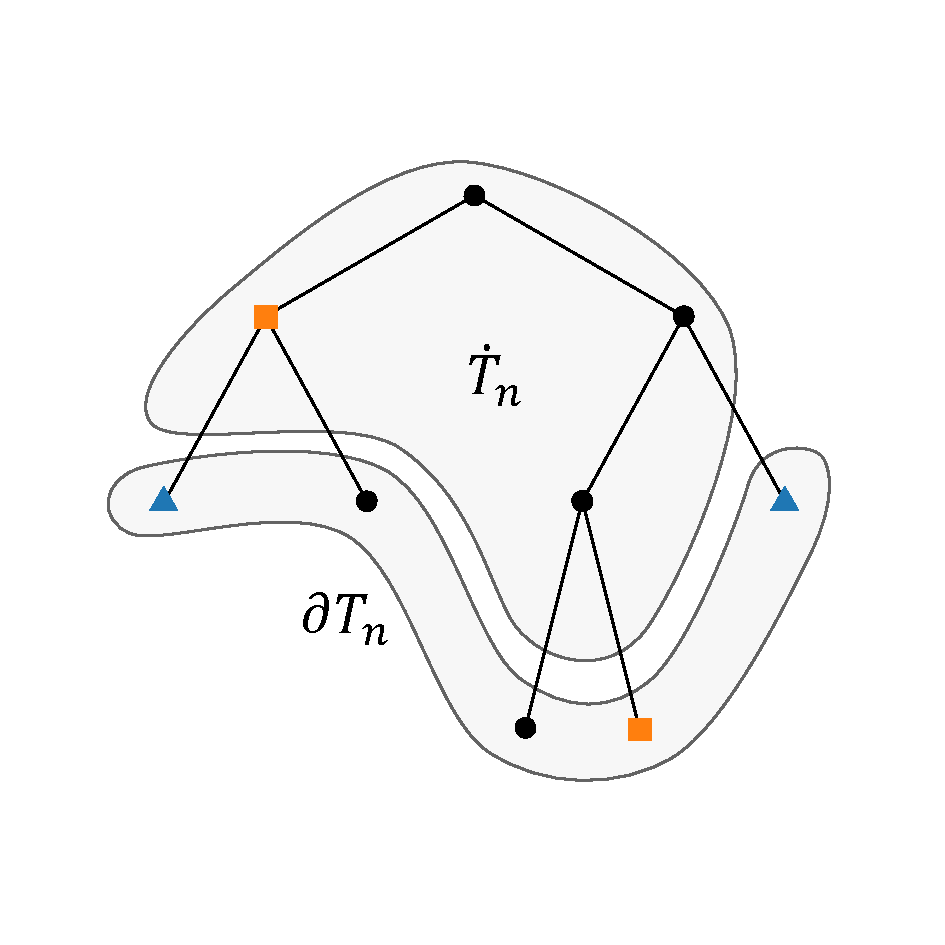
\includegraphics[trim={1.8cm 1.2cm 1.9cm 1.2cm}, clip,width=0.44\linewidth]{img/tree_1}
	\hfill
	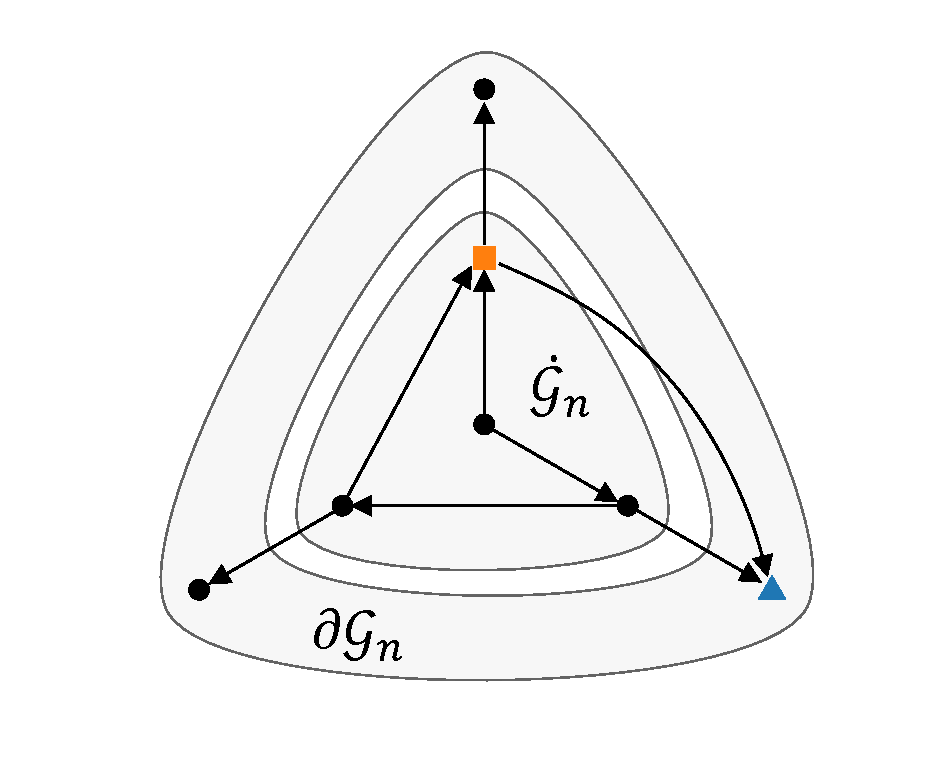
\includegraphics[trim={1.8cm 1.2cm 1.9cm 0.9cm}, clip,width=0.44\linewidth]{img/graph_1}
	\caption{Depiction of the tree $\Tau_n$ (left) and the graph $\cG_n$ (right) built with the same observed transitions. In the tree, two nodes of the same colour lead to the same state.}
	\label{fig:structures}
\end{figure}

In a tree, a node of depth $h$ represents a sequence of actions $a\in A^h$. The \textit{root} of the tree corresponds to the empty action sequence, and hence to the initial state $s_0\in S$. At iteration $n$, we denote the current tree as $\Tau_n$. Borrowing notations from topology, we denote its set of internal nodes as $\inte{\Tau}_n$ and its set of external nodes (the leaves) as $\ext{\Tau}_n$. Note that since the MDP is deterministic, a sequence of action $a$ is associated with its final state denoted $s(a)$, but this association is not one-to-one: several sequences of action can lead to the same state, which will be represented several times in the tree.

In a graph, the nodes represent states $s\in S$, and the edges represent transitions between states. The \textit{source} of the tree corresponds to the initial state $s_0$. At iteration $n$, we denote the current graph as $\cG_n$, its set of internal nodes as $\inte{\cG}_n$ and its set of \textit{sinks} as $\ext{\cG}_n$.

Both structures are built iteratively from a single starting node, by selecting an external node (leaf or sink) to \emph{expand}. The expansion of a node $a$ or $s$ refers to calling the generative model to sample the reward $r$ and next state $s'$ for each action $a\in A$, and adding child nodes to the data structure. In a tree, the expansion of a node $a\in A^h$ always lead to the creation of new leaf nodes that represent the suffix sequence of action $ab\in A^{h+1},\, b\in A$. In contrast, in a graph the next state $s'$ reached from $s,a$ might already be present in $\cG_n$, in which case we add the edge between $s$ and $s'$ without creating a new node.
These data structures can be used to store information about the MDP, such as the transitions and rewards $r(s, a)$, or other informations useful for planning.


\subsection{Optimistic planning}

A planning algorithm is typically composed of two main rules:
\begin{enumerate*}[label=(\roman*)]
	\item A \emph{sampling rule}, that selects promising transitions to simulate at each iteration $n$;
	\item A \emph{recommendation rule}, that recommends a first good action to take.
\end{enumerate*}
%The pseudo-code of generic planning algorithm is provided in \Cref{alg:generic}.
%\begin{algorithm}
%	\caption{A generic planning algorithm}
%	\label{alg:generic}
%	\DontPrintSemicolon
%	\For{each iteration $n$}{
%		Select the node $\hat{a}_n$ (or $\hat{s_n}$) to expand according to the \textbf{sampling rule}.\;
%		\For(\Comment*[f]{Node expansion}){action $a\in A$}{
%			Simulate the transition $r, s' \sim \probability{r, s' \condbar s, a}$ from the generative model.\;
%			Insert the observed transition to the data structure accordingly.
%		}
%	}
%	\Return the recommended action $a_{n}$ according to the \textbf{recommendation rule}.\;
%\end{algorithm}
These rules can be chosen with the goal of minimising the simple regret $r_n$.
A popular approach is to follow the principle of \emph{Optimism in the Face of Uncertainty} (OFU) \citep[see][]{Munos14}, which consists in exploring the option that maximises an upper-bound of the true objective. In the context of planning, it has been applied by forming bounds on the value function $V$.

\begin{definition}[Value bounds]
\paragraph{\textbf{On trees.}} We denote by $L:\Tau_n \rightarrow \Real$ and  $U:\Tau_n \rightarrow \Real$ a lower-bound and upper-bound for the state value $V$ defined on the tree $\Tau_n$, such that
\begin{equation*}
    \forall a\in\Tau_n, \qquad L(a) \leq V(s(a)) \leq U(a).
\end{equation*}

\paragraph{\textbf{On graphs.}} Likewise, we denote by $\cL:\cG_n \rightarrow \Real$ and  $\cU:\cG_n \rightarrow \Real$ a lower-bound and upper-bound for the state value $V$ defined on the graph $\cG_n$, such that
\begin{equation*}
\forall s\in\cG_n, \qquad \cL(s) \leq V(s) \leq \cU(s).
\end{equation*}
\end{definition}

Following the OFU principle, at iteration $n$ we must leverage available information to design an upper-bound $U_n$ (or $\cU_n$) on $V$ as tight as possible. Then, in order to select an promising external node to expand, the sampling rule starts from the root (or source) and follows the optimistic strategy of always selecting the action which maximises $U_n$ (or $\cU_n$), until reaching an optimistic leaf (or sink) to expand. This strategy was used in \citep[e.g.][]{Kocsis06UCT, Hren2008optimistic, Bubeck2010open, Busoniu2012optimistic}.

For instance, since we assume that the rewards are bounded in [0, 1], trivial bounds on $V(s)$ are
$0 \leq V(s) \leq V_{\max} \eqdef {1}/({1-\gamma})$. But these trivial bounds are the same for every node, which makes them non-informative, and do not make use of the observed information. However, they can be used as a valid starting point. Every observed transition stored in the graph / can then be used to tightened these bounds, by using the Bellman Optimal operator.

\begin{definition}[Bellman Optimal operator]
	\label{def:bellman}
	\paragraph{\textbf{On trees.}} We define the Bellman Optimal operator $B_n$ on the tree $\Tau_n$ as:
	\begin{equation}
	\label{eq:bellman-tree}
	B_n(f)(a) \eqdef \begin{cases}
	\max_{b\in A} r(s(a), b) + \gamma f({ab})
	& \text{if $a\in\inte{\Tau}_n$.} \\
	f(a) & \text{if $a\in\ext{\Tau}_n$;}
	\end{cases}
	\end{equation}
	
	\paragraph{\textbf{On graphs.}} Likewise, we define the Bellman Optimal operator $\cB_n$ on the graph $\cG_n$ as:
	\begin{equation}
	\label{eq:bellman-graph}
	\cB_n(f)(s) \eqdef \begin{cases}
	\max_{b\in A} r(s, b) + \gamma f(T(s,b))
	& \text{if $s\in\inte{\cG}_n$.} \\
	f(s) & \text{if $s\in\ext{\cG}_n$;}
	\end{cases}
	\end{equation}
	The updates of both Bellman operators are depicted in \Cref{fig:bellman}.
\end{definition}

%\begin{remark}
%	For ease of notation, we will sometimes drop the $n$ index on $B$ and $\cB$ when it is non-ambiguous.
%\end{remark}


\begin{figure}[tp]
	\centering
	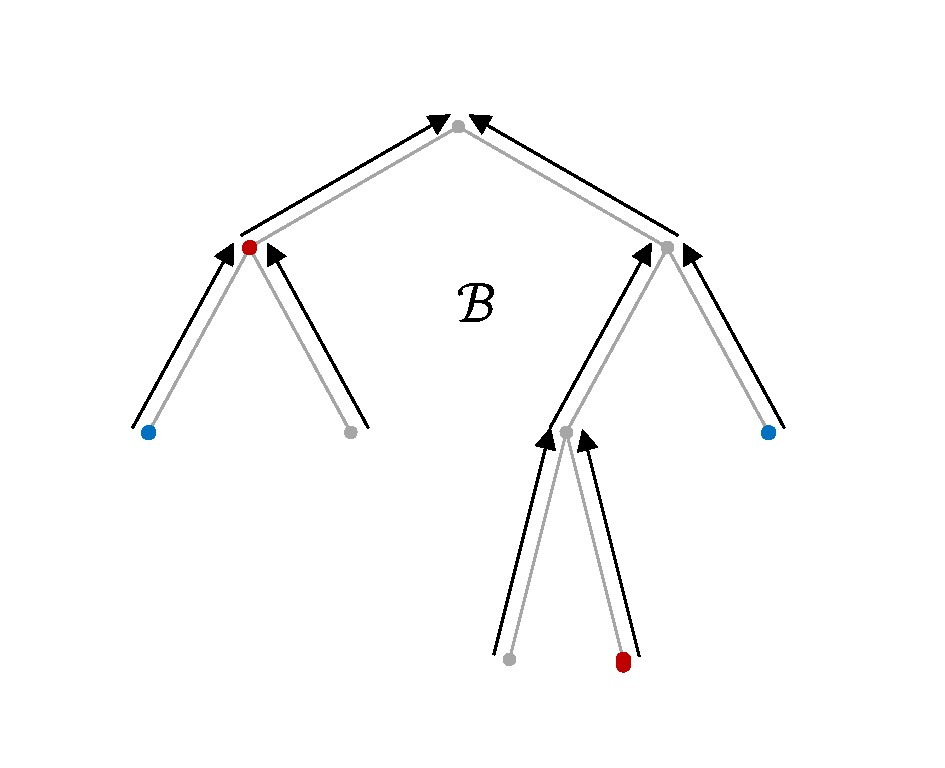
\includegraphics[trim={1.8cm 1.4cm 1.9cm 1.9cm}, clip,width=0.42\linewidth]{img/tree_2}
	\hfill
	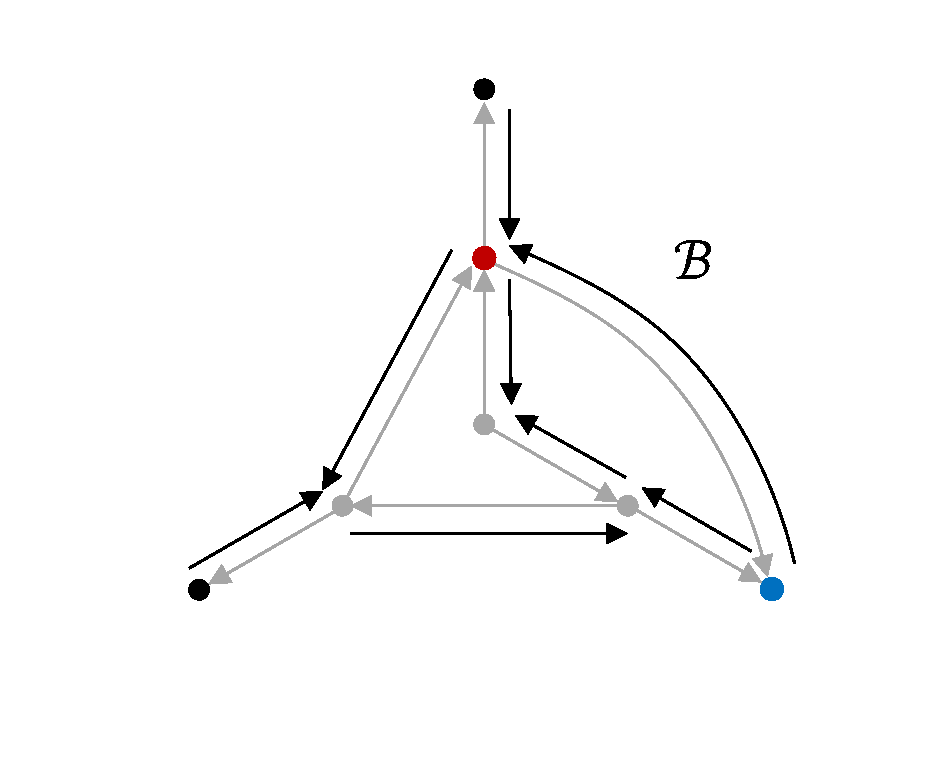
\includegraphics[trim={1.8cm 2.6cm 1.9cm 1.3cm}, clip,width=0.46\linewidth]{img/graph_2}
	\caption{Depiction of the Bellman backup operators $B$ (left) and $\cB$ (right). Notice that $B$ only propagates information upward in the tree.}
	\label{fig:bellman}
\end{figure}

\citet{Hren2008optimistic} used this Bellman operator $B_n$ in their \texttt{OPD} algorithm to define a pair of bounds $(L_n,\, U_n)$ at each iteration $n$. They use trivial bounds at the leaves, and backup these estimates up to the root by iteratively applying $B_n$. We can show that, under a \textit{monotonicity} condition (satisfied by the trivial bounds $0$ and $V_{max}$), applying $B_n$ can only tighten a bound and converges in a finite time.

\begin{definition}[Monotonicity]
	A pair of bounds ($L$, $U$) or $(\cL, \cU)$ is \emph{monotonic} if they are respectively non-decreasing and non-increasing along transitions:
	\begin{align*}
	\forall a\in{\Tau}_n, \quad & L(a) \leq B_n(L)(a), & U(a) & \geq B_n(U)(a)\\
	\forall (s)\in\inte{\cG}_n, \quad &\; \cL(s) \leq \cB_n(\cL)(s),&   \cU(s) & \geq \cB_n(\cU)(s)
	\end{align*}
\end{definition}

\begin{lemma}[Properties of $B_n$]
	\label{lem:properties-b-tree}
	\begin{enumerate}[label=(\roman*)]
		\item $B_n$ preserves monotonicity and tightens monotonic bounds: $$
		L \leq B_n(L) \leq V \leq B_n(U) \leq U;
		$$
		\item $(B_n^k)_k$ converges in a finite time $d_n$, where $d_n$ is the depth of $T_n$. 
	\end{enumerate}
\end{lemma}
This enables \citet{Hren2008optimistic} to define non-trivial valid bounds on $V$:
\begin{align}
L_n = B_n^{d_n}(0), \qquad U_n = B_n^{d_n}(V_{\max}).
\end{align}
and their \texttt{OPD} algorithm, described in \Cref{alg:opd}. Likewise, we have:
\begin{lemma}[Properties of $\cB_n$]
	\label{lem:properties-b-graph}
	\begin{enumerate}[label=(\roman*)]
		\item $\cB_n$ preserves monotonicity and tightens monotonic bounds: $$
		\cL \leq \cB_n(\cL) \leq V \leq \cB_n(\cU) \leq \cU;
		$$
		\item $\cB$ is a $\gamma$-contraction, and we denote $\cB_n^{\infty} \eqdef \lim_{k\rightarrow \infty} \cB_n^k$.
	\end{enumerate}
\end{lemma}
which motivates us to propose \Cref{alg:gbop-d}, following the approach of \Cref{alg:opd} adapted to a graph structure. Though the two algorithms share a similar design, we claim that using graphs provides substantial theoretical and practical performance improvements, and back up this statement in \Cref{sec:analysis,sec:experiments}.

\begin{algorithm}[th]
	\caption{The \emph{Optimistic Planning of Deterministic Systems} (\OPD) algorithm from \citep{Hren2008optimistic}.}
	\label{alg:opd}
	\DontPrintSemicolon
	\For{each iteration $n$}{
		Compute the bounds $L_n = B_n^{d_n}(0)$ and $U_n = B_n^{d_n}(V_{\max})$.\; 
		
		$\hat{a}_n$ = $\emptyset$\;
		\While{$\hat{a}_n\in\inte{\Tau}_n$}{
			$\hat{a}_n\gets \displaystyle\argmax_{a'\in \hat{a}_n A} r(a') + \gamma U(a')$ \Comment*[r]{Optimistic sampling rule}
		}
		\For(\Comment*[f]{Node expansion}){action $a\in A$}{
			Simulate $r, s' \sim \probability{r, s' \condbar s(\hat{a}_n), a}$.\;
			Add a new leaf $\hat{a}_n a$ to $\Tau_{n+1}$, with associated reward $r$.
		}
	}
	\Return $\displaystyle\argmax_{a\in A} r(s, a) + \gamma L_n(a)$. \Comment*[r]{Conservative recommendation rule}\;
\end{algorithm}

\begin{algorithm}[th]
	\caption{Our \emph{Graph-Based Optimistic Planning for Deterministic systems} (\GBOPD) algorithm.}
	\label{alg:gbop-d}
	\DontPrintSemicolon
	\For{each iteration $n$}{
		Compute the bounds $\cL_n = \cB_n^{\infty}(0)$ and $\cU_n = \cB_n^\infty(V_{\max})$.\; 
		
		$\hat{s}_n$ = $s_0$\;
		\While{$\hat{s}_n\in\inte{\cG}_n$}{
			$\hat{s}_n\gets \displaystyle\argmax_{s'} r(s, a) + \gamma \cU_n(s')$ \Comment*[r]{Optimistic sampling rule}
		}
		\For(\Comment*[f]{Node expansion}){action $a\in A$}{
			Simulate $r, s' \sim \probability{r, s' \condbar s, a}$.\;
			Get or create the node $s'$ in $\cG_{n+1}$, and add the transition $(s,a) \rightarrow s', r$.
		}
	}
	\Return $\displaystyle\argmax_{a\in A} r(s,a) + \gamma \cL_n(s(a))$. \Comment*[r]{Conservative recommendation rule}
\end{algorithm}

\section{Analysis}
\label{sec:analysis}

Comparing \OPD and \GBOPD directly is difficult since they do not involve the same structure, which implies implicit differences in their behaviours. Studying them under a common framework would make these differences explicit. In order to leverage the analysis of the \texttt{OPD} algorithm by \citet{Hren2008optimistic}, we frame \GBOPD as a tree-based planning algorithm. To account for the distinction between the operators $B$ and $\cB$, we represent $\cB$ as tree backup $B$ augmented with \emph{merge} operator $M$ which enforces that nodes with similar states share the same value.

\subsection{Background on the sample complexity of \OPD}

First, we recall the analysis of \citet{Hren2008optimistic}. We start by introducing some notations.

\begin{definition}[Sequence values]
The value of a finite \textbf{sequence} of actions $a\in A^h$ is:
\begin{equation*}
\label{eq:state_value}
    V(a) = R(s_0,a) + \gamma^{h} V(s(a)),
\end{equation*}
where $R(s, a) = \sum_{t=0}^{h-1} \gamma^t r(a_{1:t})$ is the return of the sequence $a$ starting from the state $s$.
\end{definition}

This enables to define a measure of the difficulty of a planning problem.

\begin{definition}[Difficulty measure]
We define the near-optimal branching factor $\hlrb{\kappa}$ of an MDP as
\begin{equation}
\hlrb{\kappa = \limsup_{h\rightarrow\infty} |\hlrb{\Tau_h^\infty}|^{1/h}} \in [1, K]
\end{equation}
where $\Tau^\infty_h = \displaystyle \left\{a\in A^h: V^\star-V(a) \leq \frac{\gamma^h}{1-\gamma}\right\}$ is the subtree of near-optimal nodes.
\end{definition}

This problem-dependent measure $\hlrb{\kappa}$ is the branching factor of the subtree $T^\infty$ of near-optimal nodes that can be sampled by \OPD, and acts as an effective branching factor as opposed to the true branching factor $K$. When $\kappa$ is small, fewer nodes need to be explored at a given depth, which means that the planner will be able to plan deeper for a given budget $n$. Thus, it directly impacts the simple regret that can be achieved by \OPD when run on a given MDP.


\begin{theorem}[Regret bound of \citealt{Hren2008optimistic}]
\label{thm:regret-opd}
The \Cref{alg:opd} enjoys the following regret bound:
\begin{align*}
\quad r_n = \tilde{\cO}\left( n^{-\log \frac{1}{\gamma}/\hlrb{\log\kappa}}\right).
\end{align*}
where $f_n = \tilde{\cO}(n^{-\alpha})$ means that for any $\alpha'<\alpha$, $f_n = \cO(n^{-\alpha'}).$
%where $f_n = \tilde{\cO}(g_n)$ means that $f_n$ is a $\cO(g_n)$ up to an \emph{infinitesimal} polynomial factor: for any $\alpha>0$, $f_n = {\cO}(g_n n^{\alpha}).$
\end{theorem}


$\hlrb{\kappa}$ is typically small in problems where there is one clearly identified optimal trajectory, of which any deviation can be quickly dismissed as suboptimal. Conversely, $\kappa$ is large when there are many suboptimal trajectories that cannot be distinguished easily based on their values, which requires the uniform exploration of the entire tree $T$ with its original branching factor $K$.

\oam{Recall some examples from literature.}
\oam{Add discussion regarding literature scarcity on the topic}

\subsection{Motivation for an improved regret bound}

We start by reformulating the sampling rule used for the \texttt{OPD} algorithm. To that end, notice that when some bounds $(L,\,U)$ on the state values $V(s(a))$ are available, they also induce bounds $(\overline{L},\, \overline{U})$ on values $V(a)$ of sequences of actions $a\in A^h$ defined as:
\begin{equation*}
%\label{eq:sequence_value}
\underbrace{R(a) + \gamma^{h} L(a)}_{\overline{L}(a)} \leq V(a) \leq \underbrace{R(a) + \gamma^{h} U(a)}_{\overline{U}(a)}
\end{equation*}


One can easily see that, since the $(L_n,\,U_n)$ used in the optimistic sampling rule described in \Cref{alg:opd} are invariant by $B_n$ by definition, this rule can be equivalently expressed as:
\begin{equation}
\label{eq:sampling_rule}
\hat{a}_n \in \argmax_{a\in\ext{\Tau}_n} \overline{U}_n(a).
\end{equation}
Likewise, the conservative recommendation rule returns the first action of:
\begin{equation}
\label{eq:recommendation_rule}
a_n \in \argmax_{a\in\ext{\Tau}_n} \overline{L}_n(a)
\end{equation}


As shown in \Cref{fig:bellman}, in a tree the Bellman operator $B_n$ only propagates the information upward, and the leaves cannot be updated. Thus, $U_n = B_n^{d_n}(V_{\max})$ and $V_{\max}$ coincide on $\ext{\Tau}_n$ which means that the sampling rule of \texttt{OPD} can be summarized as using \eqref{eq:sampling_rule} with the trivial upper-bound $U_n = V_{\max}$.
Likewise, the recommendation rule simply uses \eqref{eq:recommendation_rule} with the trivial lower-bound $L_n = 0$. Thus, \texttt{OPD} amounts to simply using the trivial bound $(0,\, V_{\max})$ on leaf nodes, and does not make use of all the available information in $\Tau_n$ to improve these bounds.

Assume that we instead had access to some tighter bounds $(L,\,U)$ provided by an oracle: $$0\leq L\leq V\leq U\leq V_{\max}.$$
\begin{definition}[A finer difficulty measure]
We define the near-optimal branching factor \emph{according to the bounds $(L,\,U)$} as 
\begin{equation}
\hlbb{\kappa(L,U) \eqdef \limsup_{h\rightarrow\infty} \left|\Tau_h^\infty(L,U)\right|^{1/h}}\in(1, K], 
\end{equation}
where
$ \displaystyle
     {\Tau_h^\infty(L,U)}=\left\{a\in A^h: V^\star - V(a)\leq \gamma^{h}(U(a)-L(a))\right\}.
$
\end{definition}

\begin{lemma}
\label{lem:shrink}
This branching factor shrinks as the bounds $(L,\,U)$ get tighter:
\[L_2\leq L_1\leq V\leq U_1\leq U_2\implies \kappa(L_1,U_1) \leq \kappa(L_2,U_2).\]
In particular, $\hlbb{\kappa(L,U)} \leq \hlrb{\kappa}$.
\end{lemma}

\begin{theorem}
\label{thm:regret-bound-U}
Let $L \leq V\leq U$ monotonic bounds, then planning with $L$ and $U$ in \eqref{eq:sampling_rule} and \eqref{eq:recommendation_rule} yields the following simple regret bound:
\begin{equation*}
r_n = \tilde{\cO}\left(n^{-\log \frac{1}{\gamma}/\hlbb{\log \kappa(L,U)}}\right).
\end{equation*}
\end{theorem}


This theorem states that we can potentially improve the performance of the planning algorithm if we manage to find bounds $(L,\, U)$ that are tighter than the trivial ones at the leaves $\ext{\Tau_n}$, but it does not explain how to obtain such bounds. In the next subsection, we describe a method to build at each planning iteration $n$ a sequence of increasingly tight bounds $(L^k,\, U^k)$. The corresponding regret bound, our main result, is stated in \Cref{thm:regret-gbop-t}.


\subsection{Merging the states}

In order to reproduce the behaviour of \Cref{alg:gbop-d} on a tree structure, we rely on two observations: \begin{enumerate*}[label=(\roman*)]
	\item in $\cG_n$, all paths leading to a single state $s$ share the same bounds $\cL(s)$ and $\cU(s)$;
	\item in $\cG_n$, expanding a node $s$ simultaneously expands all the paths leading to this node.
\end{enumerate*}
They are implemented on top of \Cref{alg:opd} through the introduction of two additional operators: $M$ (\Cref{def:merge}) and $P$ (\Cref{prop:pruning}),  illustrated in \Cref{fig:operators}.

\begin{definition}[Merge operator $M_n$]
	\label{def:merge}
If several sequences $a'\in\Tau_n$ all lead to the same state $s$, their respective bounds must hold simultaneously. We introduce the merge operator $M_n$ as:
    \begin{align}
    \label{eq:merge}
        \forall a\in\mathcal{T}_n, \qquad &M_n^-(L)(a) = \max_{a'\in N_n(a)} L(a'),\qquad M_n^+(U)(a) = \min_{a'\in N_n(a)} U(a'),                                   
    \end{align}
    where $N_n(a)$ is the set of \emph{neighbours} of a sequence of action $a\in A^h$, that lead to the same state:  $N_n(a) = \{a'\in\Tau_n: s(a)=s(a')\}$.
\end{definition}

\begin{remark} For ease of notation, we sometimes refer to $M_n^-$ and $M_n^+$ as a single merge operator $M_n$, that acts as $M_n^-$ on lower-bounds and $M_n^+$ on upper-bounds.
\end{remark}

\begin{figure}[th]
	\centering
	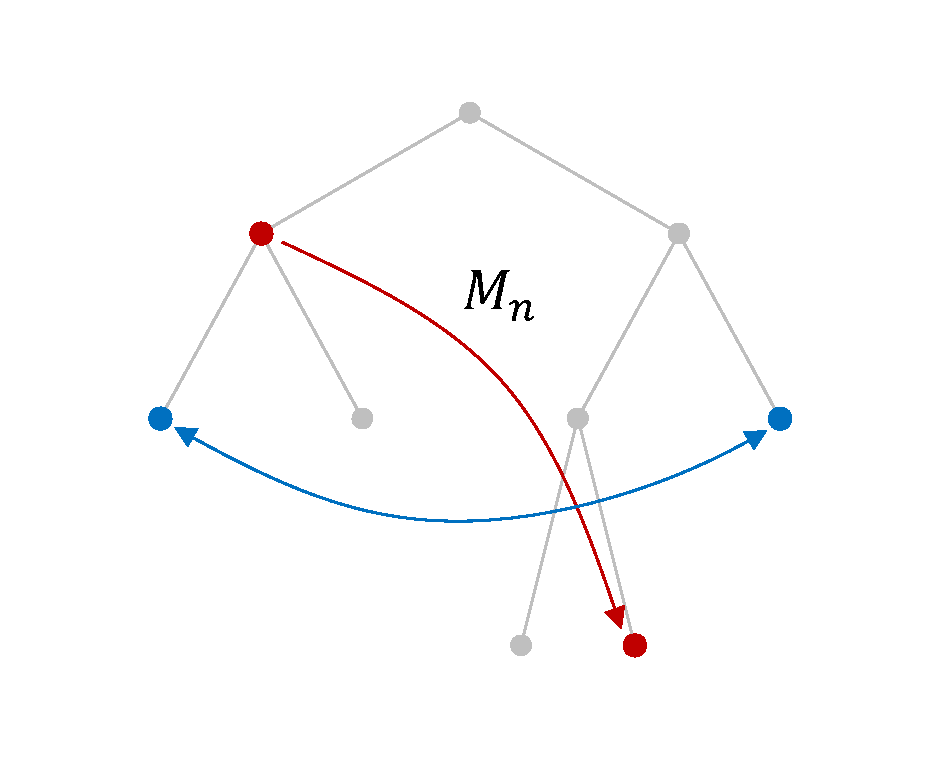
\includegraphics[trim={1.8cm 1.4cm 1.1cm 1.1cm}, clip,width=0.42\linewidth]{img/tree_3}
	\qquad
	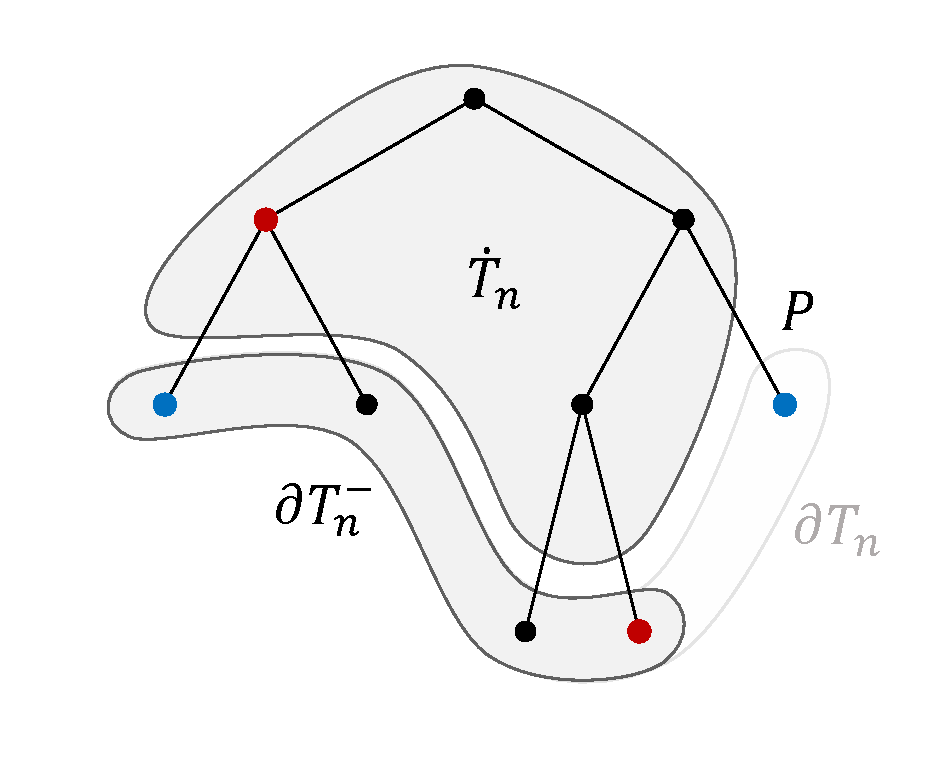
\includegraphics[trim={1.8cm 1.4cm 1.1cm 1.1cm}, clip, width=0.42\linewidth]{img/tree_4}
	\caption{\textbf{Left:} The merge operator $M_n$. Any node of $\Tau_n$ can be updated, and in particular its leaves $\ext{\Tau}_n$. \textbf{Right:} The pruning operator $P$. A leaf verifying the criterion of \Cref{prop:pruning} is removed from the set of candidates to expansion.}
	\label{fig:operators}
\end{figure}

We now argue that the introduction of this merge operator $M_n$ enables to reproduce the behaviour of $\cB_n$ on a tree.

\begin{definition}[Bounds equivalence]
	We say that a bound $U\in (T_n)^\Real$ is \emph{equivalent} to a bound $\cU \in (\cG_n) ^\Real $ if for all sequence $a\in A^*$, $U(a) = \cU(s(a))$.
\end{definition}

\begin{proposition}[``$\cB = MB$"]
	\label{prop:b-eq-mb}
	If $U$ and $\cU$ (resp. $L$ and $\cL$) are equivalent, then $(M_n^+B_n)(U)$ and $\cB_n(\cU)$ (resp. $(M_n^-B_n)(L)$ and $\cB_n(\cL)$) are also equivalent.
\end{proposition}

Since in \Cref{alg:gbop-d} the bounds $(\cL_n, \cU_n)$ are defined as a fixed-point iteration of $\cB_n$, starting from the trivial bounds $(0,\, V_{\max})$, we translate this definition in the context of trees with an alternating procedure of backups $B_n$ and merges $M_n$. At iteration $n$ we define the bounds
\begin{equation}
\label{eq:tree-bounds}
L_n = (M_n^- B_n)^\infty(0), \qquad
U_n = (M_n^+ B_n)^\infty(V_{\max}),
\end{equation}
Note that $L_n, U_n$ are well defined, since:
\begin{lemma}[Properties of $M_nB_n$]
	\label{lem:properties-mb}
	\begin{enumerate}[label=(\roman*)]
		\item $M_n B_n$ preserves monotonicity and tightens monotonic bounds;
		\item $M_n B_n$ a $\gamma$-contraction.
	\end{enumerate}
\end{lemma}

By \Cref{prop:b-eq-mb}, the bounds $(\cL_n, \cU_n)$ and $(L_n, U_n)$ are respectively equivalent, and the optimistic sampling rule will sweep the same sequences of actions. It remains to deal with the second observation (ii): in \Cref{alg:gbop-d}, expanding a node simultaneously expands all the sequences of actions leading to this node. We could proceed similarly in $T_n$, by automatically expanding leaves that represent the same state as an internal node, but that would result in infinite trees whenever a loop is observed. We instead opt for the alternative solution of pruning any leaf $a$ that constitutes a suboptimal path to $s(a)$.


\begin{proposition}[Pruning operator $P$]
	\label{prop:pruning}
	Let $a_1,a_2\in\Tau_n$ such that state $s(a_1) = s(a_2) = s$ and $U = M(U) \geq V$ an aggregated upper-bound. 
	\begin{equation}
	\label{eq:pruning}
	\text{If } h(a_2) \geq h(a_1) \text{ and } \overline{U}(a_2) \geq \overline{U}(a_1)
	\text{, then }V(a_2) \geq V(a_1)
	\end{equation}
	
	In particular, there is no need to ever expand the node $a_1$. We propose that at each step, we detect such pairs $a_1, a_2$. Whenever $a_1$ is a leaf, we can remove it from the set $\ext{\Tau}_n^-\subset \ext{\Tau}_n $ of candidates for expansion.
\end{proposition}


%\begin{corollary}
%	The nodes $\hat{a}_n$ selected by the sampling rule \eqref{eq:sampling_rule} using the merged bounds \eqref{eq:tree-bounds} lead to the same states %$s(\hat{a}_n)$
%	as those ($\hat{s}_n$) sampled by \Cref{alg:gbop-d}.
%\end{corollary}


We finally describe in \Cref{alg:gbop-t} the tree version \GBOPD.

\begin{algorithm}[H]
	\caption{Tree version of \Cref{alg:gbop-d}}
	\label{alg:gbop-t}
	\DontPrintSemicolon
	\For{iteration $n$}{
		Compute $L_n = (M_n^-B_n)^\infty(0)$, $U_n = (M_n^+B_n)^\infty(V_{\max})$ with \eqref{eq:bellman-tree}, \eqref{eq:merge}.\;
		Select the optimistic sequence of actions $\hat{a}_{n}$ from \eqref{eq:sampling_rule} in $\ext{T_n}^-$.\;
		\For{action $a\in A$}{
			Add the child $\hat{a}_{n}a$ to the tree $\Tau_{n+1}$ and simulate its reward.
		}
		Prune the tree: $\ext{\Tau}_{n+1}^- = P(\ext{\Tau}_{n+1})$.\;
	}
	\Return the recommendation $a_{n+1}$ from \eqref{eq:recommendation_rule}.\;
\end{algorithm}

\subsection{Main result}

In \Cref{thm:regret-bound-U}, we assumed that some bounds $(L,\,U)$ were revealed by an oracle and available from the onset for planning. In \Cref{alg:gbop-t}, we instead built a \emph{sequence} of bounds $(L_n,U_n)_{n\geq 0}$ \eqref{eq:tree-bounds} that is non-increasing in the sense of inclusion, i.e. $0\leq \dots\leq L_{n-1}\leq L_n\leq V\leq U_n\leq U_{n-1}\leq \dots\leq V_{\max}$.

We can consider the sequence $\kappa_n = \kappa(L_n, U_n)$. It is non-increasing and lower-bounded by $1$, thus converges. Let $\hlgb{\kappa_\infty = \lim_{n\rightarrow\infty} \kappa(L_n, U_n)} \in[1,K]$.

\begin{theorem}
\label{thm:regret-gbop-t}
\Cref{alg:gbop-t} enjoys the following regret bound, with $\hlgb{\kappa_\infty} \leq \hlrb{\kappa}$: 
\begin{align*}
r_n = \tilde{\cO}\left(n^{-\log \frac{1}{\gamma}/\hlgb{\log \kappa_\infty}}\right).
\end{align*}
\end{theorem}

Intuitively, $\kappa_\infty$ should be much lower than $\kappa$ in problems where trajectories overlap a lot. For instance, it will be the case for problems where two actions cancel each-other out (e.g. moving left or right), or are commutative (e.g. placing pawns on a board game). However, this is merely an intuition. So far we have not proven the existence of problem instances such that $\hlgb{\kappa_\infty} < \hlrb{\kappa}$, which is a legitimate concern since their non-existence would make \Cref{thm:regret-gbop-t} trivial and uninformative.

\subsection{Illustrative example}

We consider a toy MDP $\cM$ shown in \Cref{fig:mdp}. The transitions are described visually while the rewards are defined as follows: let $0\leq r^\star\leq \gamma$, and $ r^- = r^\star - \frac{\gamma}{1-\gamma} S$, $r^+ = r^\star + S$ with $S = r^\star\left(\frac{1}{\gamma} - 1\right).$ Note that the choice ensures that $r^\star, r^-, r^+$ and $S$ are all in $[0, 1]$.

\begin{figure}[htp]
    \centering
    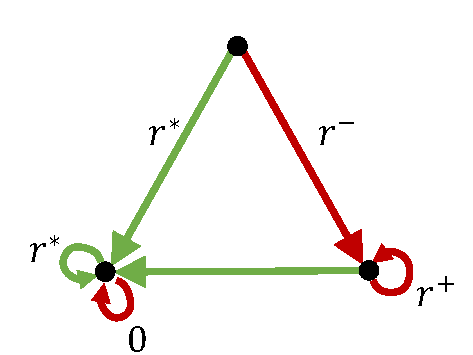
\includegraphics[trim={0.5cm 0.0cm 0.3cm 0.6cm}, clip, width=0.35\textwidth]{img/mdp.pdf}
    \caption{A toy MDP with three states and $K \geq 2$ actions. We start in the top state. The first action $a_1$ is represented by \textcolor{OliveGreen}{green} arrows, and all other actions $a_2, \dots, a_K$ are represented by \textcolor{red}{red} arrows. The rewards are shown next to the transitions.}
    \label{fig:mdp}
\end{figure}

\begin{proposition}[Comparison of branching factors]
\label{prop:illustrative-example}
The MDP $\cM$ verifies $\hlrb{\kappa = K-1}$ and $\hlgb{\kappa_\infty = 1}$.
% :
% \begin{enumerate}[label=(\roman*)]
%     \item $\hlrb{\kappa = K-1}$;
%     \item $\hlgb{\kappa_\infty = 1}$.
% \end{enumerate}
\end{proposition}
This result confirms that \Cref{thm:regret-gbop-t} is non-trivial since we exhibit a problem where $\hlgb{\kappa_\infty} < \hlrb{\kappa}$ (when $K\geq 3$), and legitimates our attempt to improve planning performances by merging the tree into a graph.


\section{Extension to Stochastic Systems}
\label{sec:stochastic}

The approach developed in \cref{sec:gbopd,sec:analysis} consists in using state similarity to tighten a pair of lower and upper bounds $(L,\,U)$ for the value function $V$. Thus, any planning algorithm that is based on such bounds can benefit from this insight, and any theoretical result based on the validity and rate of convergence of these bounds will be preserved.  

\paragraph{Confidence intervals for rewards.}

When the reward kernel $\probability{r \condbar s,a}$ is stochastic, deviation inequalities can be used to design a confidence interval $[\ell_t(s,a), u_t(s,a)]$ over its expected value $\expectedvalue\left[r | s,a\right]$. For instance, the Chernoff-Hoeffding deviation inequality was used to design confidence intervals in \citep{Kocsis06UCT,Bubeck2010open,Kaufmann2017}.
In recent works \citep{Leurent2019practical, MDPGapE2020}, the tighter Kullback-Leibler confidence interval is preferred:
\begin{align*}
u_t(s,a) &\eqdef \max \left\{v : \kl\!\big(\hat{r}_t(s,a),v\big) \leq \frac {\beta^r(n_t(s,a), n)} {n_t(s,a)} \right\},\\
\ell_t(s,a) &\eqdef\min \left\{v : \kl\!\big(\hat{r}_t(s,a),v\big) \leq \frac {\beta^r(n_t(s,a), n)} {n_t(s,a)} \right\},
\end{align*}
where $\hat{r}_t(s,a)$ is the sample mean, $\beta^r$ is an exploration function and $\kl(u,v)$ is the binary Kullback-Leibler divergence between Bernoulli distributions: $\kl(u,v) = u \log \tfrac {u} {v} + (1-u) \log \tfrac {1-u} {1-v}$.

\paragraph{Confidence region for transitions.}

Likewise, when the transition kernel $\probability{s' \condbar s,a}$ is stochastic, a confidence set on the probability vector $p(\cdot|s,a)$ can be defined as
$\cC_t(s,a) \eqdef \left\{p\in \Sigma_S :  \KL\!\big(\hp_t(\cdot|s,a),p\big) \leq \frac {\beta^p(n_t(s,a), n)} {n_t(s,a)}\right\}$,
where $\Sigma_S$ is the probability simplex over $S$, $\beta^p$ is an exploration function and $\KL(p,q)= \sum_{s \in S}  p(s) \log \tfrac{ p(s)} {{q}(s)}$ is the Kullback-Leibler divergence between categorical distributions.

\paragraph{Bellman operator with stochasticity.}

In this work, we do not discuss the tuning of $\beta^r$, $\beta^p$, but simply assume that they are chosen such that the rewards and transitions belong to their confidence regions with sufficiently high probability to obtain performance guarantees for the corresponding planning algorithm. For more details on such a choice, refer to \citep[e.g.][]{Leurent2019practical, MDPGapE2020}. We modify the \cref{def:bellman} of the Bellman operator on graphs as:

\begin{align*}
\cB_t^+(\cU)(s) &= \max_{a\in A} u_t(s,a) + \gamma \max_{p \in \cC_t(s,a)} \sum_{s'} p(s'|s,a) \cU(s'), \\
\cB_t^-(\cL)(s) &= \max_{a\in A} \ell_t(s,a) + \gamma \min_{p \in \cC_t(s,a)} \sum_{s'} p(s'|s,a)\cL(s'),
\end{align*}
for all $s\in\inte{\cG_n}$, where the maximum and minimum over these Kullback-Leibler confidence regions $\cC_t(s,a)$ can be computed as explained in \citep[Appendix A of][]{Filippi2010optimism}. Under the event that every confidence regions $[\ell_t(s,a), u_t(s,a)]$ and $\cC_t(s,a)$ are valid at time $t$, the \Cref{lem:properties-b-graph} still holds for $\cB_t^-, \cB_t^+$.

\paragraph{Structure of the planning algorithm}

In the deterministic setting, once a transition has been observed, it is known with certainty and doesn't need to be sampled ever again, which is why only external nodes $\ext{\cG_n}$ are sampled in \GBOPD. Conversely, in the stochastic setting the expected reward and transition probabilities must be estimated from samples, which implies that internal nodes $\inte{\cG_n}$ must be sampled as well. Then, it is common to adopt and episodic setting where we sample trajectories of a fixed horizon $H$, tuned depending on the budget $n$. This is the case in  \citep[e.g.][]{Kearns02SS,Kocsis06UCT,Bubeck2010open,Feldman14BRUE,Leurent2019practical,MDPGapE2020}. We also follow this scheme in our proposed \GBOP

\begin{algorithm}[ht]
	\caption{\emph{Graph-Based Optimistic Planning} (\GBOP) algorithm.}
	\label{alg:gbop}
	\DontPrintSemicolon
	\For{trajectory $m$ in $[1, M]$}{
		\For{time $t$ in $[1, H]$}{
			$n \gets (m - 1)H + h$.\;
			Compute the bounds $\cL_n = (\cB_n^-)^{\infty}(0)$ and $\cU_n = (\cB_n^+)^\infty(V_{\max})$.\; 
			$\hat{a}_t\gets \displaystyle\argmax_{a\in A} r(s_t, a) + \gamma \cU_n(s')$ \Comment*[r]{Optimistic sampling rule}
			Simulate $r_t, s_{t+1} \sim \probability{r, s_{t+1} \condbar s_t, \hat{a}_t}$.\;
			Get or create the node $s_{t+1}$ in $\cG_{n+1}$, and add an occurence of the transition $(s_t,\hat{a}_t, r_t, s_{t+1})$.
		}
	}
	\Return $\displaystyle\argmax_{a\in A} r(s,a) + \gamma \cL_n(s(a))$. \Comment*[r]{Conservative recommendation rule}
\end{algorithm}

\section{Numerical Experiments}
\label{sec:experiments}

To evaluate the practical benefits of our approach, we compare graph-based and tree-based planning algorithms in various problems.

\paragraph{Gridworld domain.}
We consider a grid in which the agent can move in $K=4$ directions. The reward function is $0$ everywhere, except in the vicinity of a goal located at $(10, 10)$, around which the reward decreases quadratically in a ball of radius $5$. %: $r(x, y) = \max(1 - \frac{1}{5^2}((x-10)^2 + (y-10)^2), 0)$. 
The \Cref{fig:deterministic-gridworld} shows number of times a state is sampled by \OPD and \GBOPD, both run with a budget $n = 5460$ and discount $\gamma=0.95$. In the absence of rewards, \OPD samples sequences of actions uniformly (in a breadth-first search manner), which --because of the dynamics structure-- results in a non-uniform occupancy of the state space $S$, where the trajectories concentrate near the starting state. In contrast, \GBOPD explores uniformly in $S$, sampling each state up to four times (from its four  neighbours), until it finds the goal vicinity and finally samples the goal location indefinitely. We reproduce the experiment in the stochastic setting by adding noise on the transitions with probability $p=10\%$, and comparing \GBOP to \MDPGapE as we show in \Cref{fig:stochastic-gridworld}. To quantify these qualitative differences, we define an exploration score: the average distance $d(s_t, s_0)$ of sampled states to the initial state (exploration) minus the distance $d(s_t, s_g)$ to the goal state (exploitation), that we show in \Cref{fig:exploration}.

\begin{figure}[ht]
	\centering
	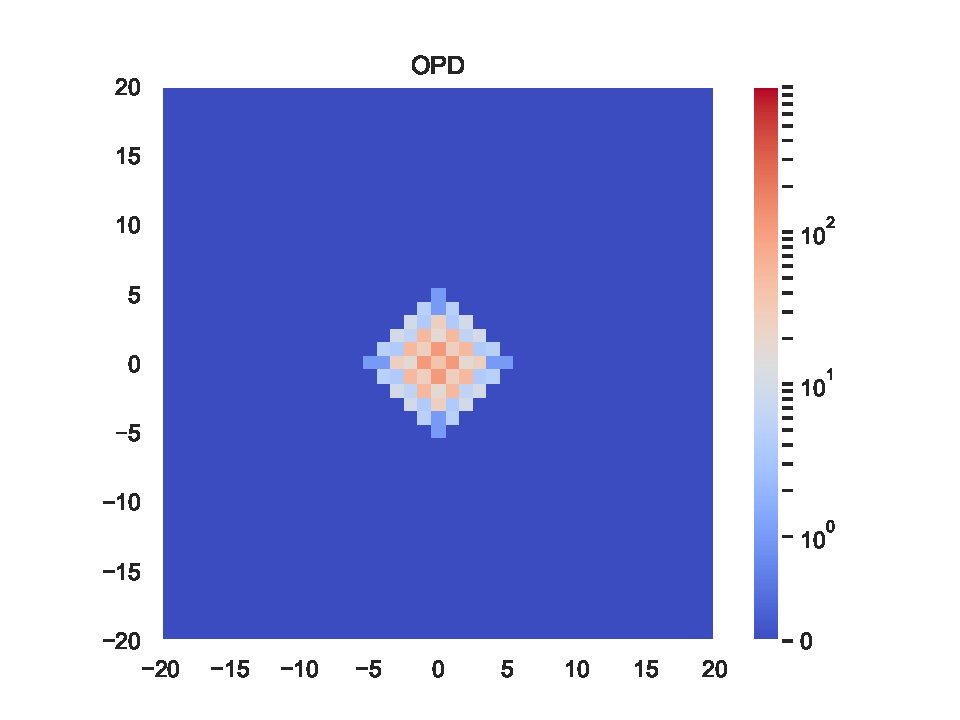
\includegraphics[trim={1.8cm 0.7cm 1.8cm 0.7cm}, clip, width=0.4\linewidth]{img/occupations_OPD.pdf}
	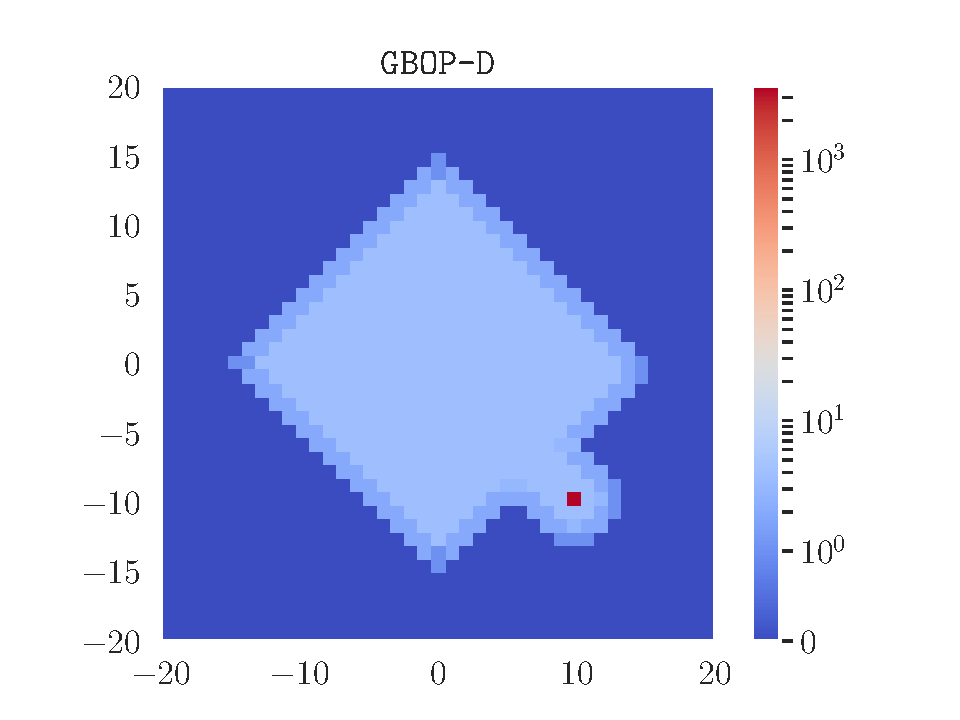
\includegraphics[trim={1.8cm 0.7cm 1.8cm 0.7cm}, clip, width=0.4\linewidth]{img/occupations_GBOP-D.pdf}
	\caption{State occupancies of two planning algorithms in a deterministic gridworld.}
	\label{fig:deterministic-gridworld}
\end{figure}
\begin{figure}[ht]
	\centering
%	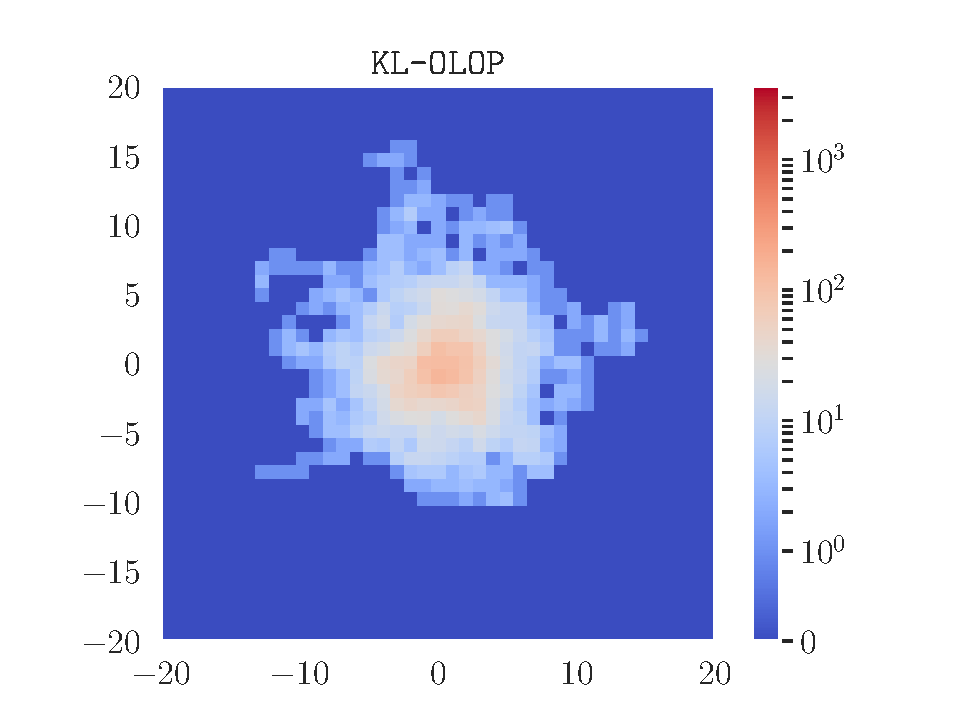
\includegraphics[trim={1.8cm 0.7cm 1.8cm 0.7cm}, clip, width=0.49\linewidth]{img/occupations_KL-OLOP.pdf}
%	\hfill
%	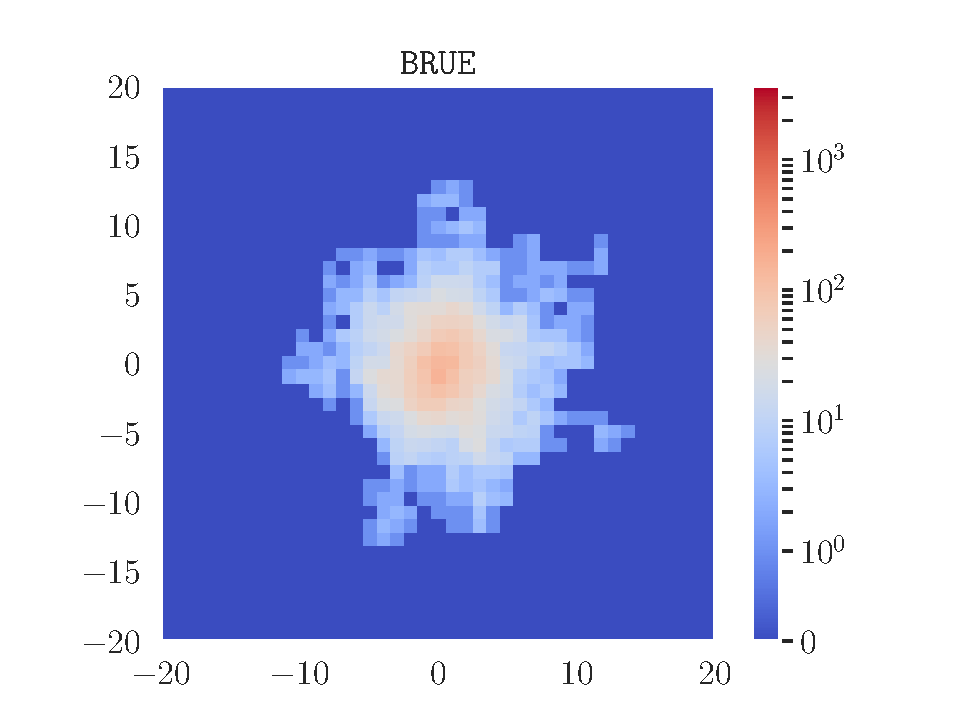
\includegraphics[trim={1.8cm 0.7cm 1.8cm 0.7cm}, clip, width=0.49\linewidth]{img/occupations_BRUE.pdf}
	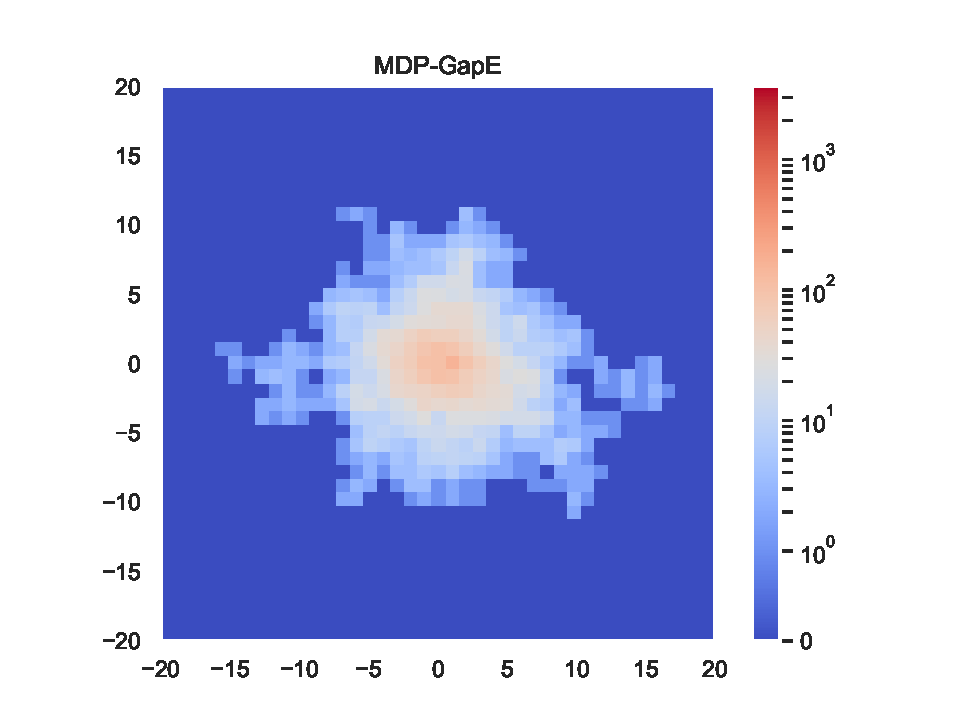
\includegraphics[trim={1.8cm 0.7cm 1.8cm 0.7cm}, clip, width=0.4\linewidth]{img/occupations_MDP-GapE.pdf}
	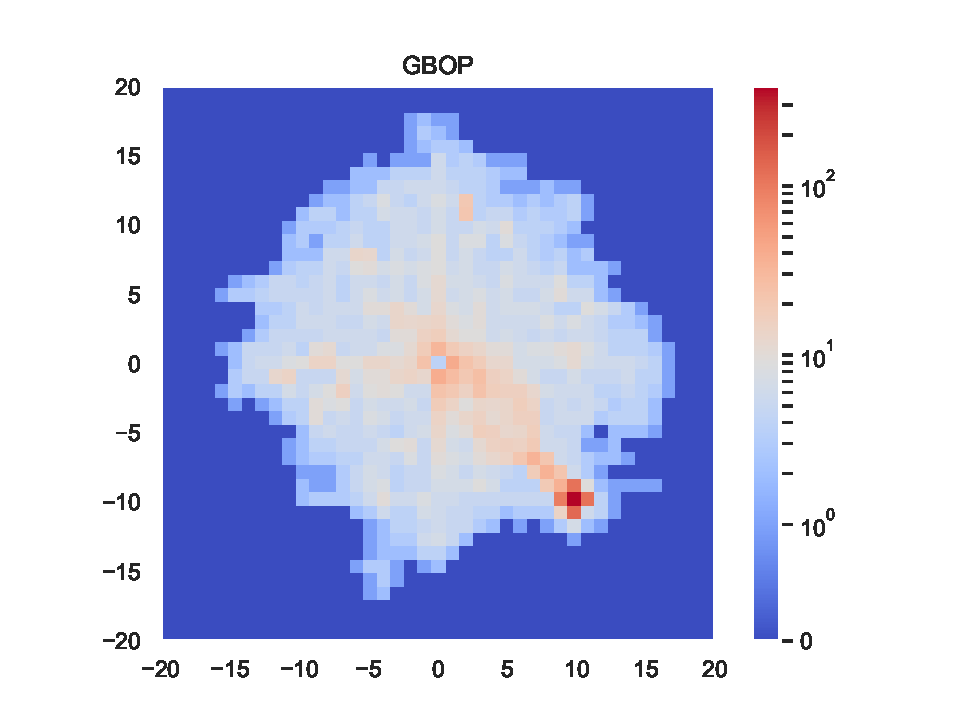
\includegraphics[trim={1.8cm 0.7cm 1.8cm 0.7cm}, clip, width=0.4\linewidth]{img/occupations_GBOP.pdf}
	\caption{State occupancies of two planning algorithms in a stochastic gridworld.}
	\label{fig:stochastic-gridworld}
\end{figure}

\paragraph{Sailing domain \citep{Vanderbei1996}.}
In a second experiment, we consider the problem of a boat sailing in $K=8$ directions to reach a goal, and enduring a cost (move duration) that depends on the direction of the wind which follows stochastic dynamics. The \Cref{fig:sailing} shows the evolution of the simple regret $r_n$ of stochastic planning algorithms with respect to the number $n$ of oracle calls. The log-log slope $\sigma$ provides an empirical measurement of the effective branching factor $\kappa_e = \exp(-\log(1/\gamma)/\sigma)$ for each algorithm. A linear regression gives $\sigma \approx-0.04$ and $\kappa_e \approx 3.6$ for BRUE, KL-OLOP, MDP-GapE. In contrast, we measure $\sigma \approx-0.25$ and $\kappa_e \approx 1.2$ for \GBOP, which suggests that our result of \Cref{thm:regret-gbop-t} might generalize to the stochastic setting.

\begin{figure}[ht]
	\centering
	\begin{subfigure}[b]{0.49\textwidth}
		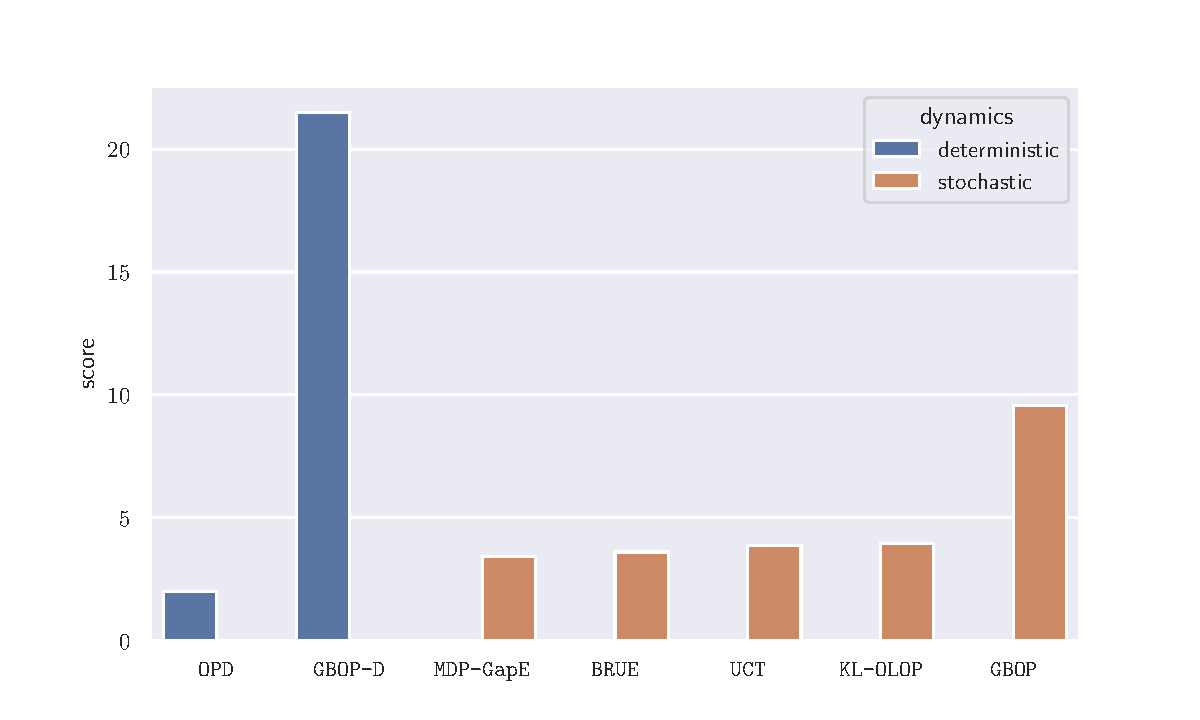
\includegraphics[trim = {0 0 0 0}, clip, width=\linewidth]{img/score.pdf}
		\caption{Exploration score in the gridworld domain}
		\label{fig:exploration}
	\end{subfigure}
	\hfill%
	\begin{subfigure}[b]{0.49\textwidth}
		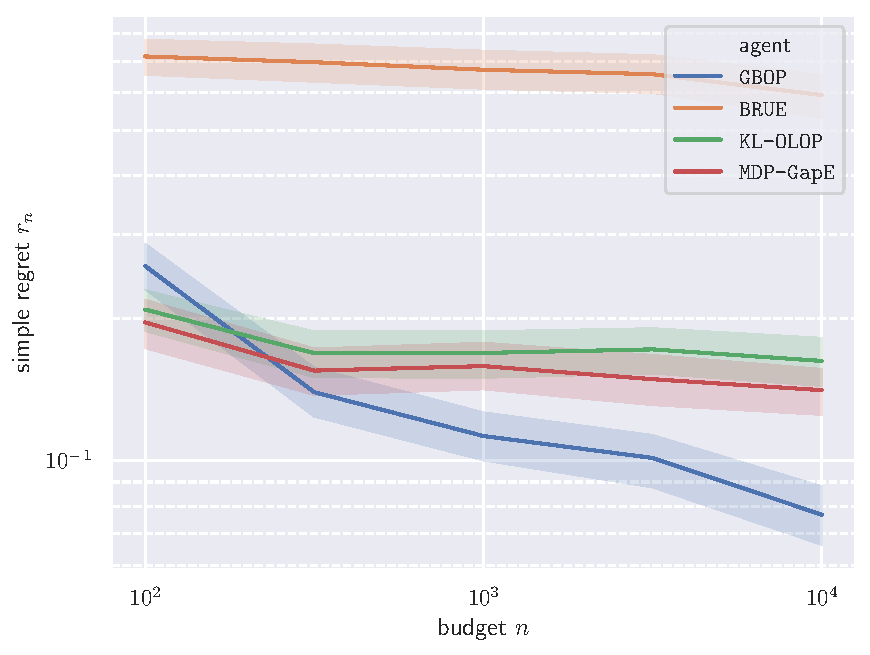
\includegraphics[trim = {0 0 0 0}, clip, width=\linewidth]{img/simple_regret.pdf}
		\caption{Simple regret $r_n$ in the sailing domain}
		\label{fig:sailing}
	\end{subfigure}
	\caption{Benchmark of planning performances.}
\end{figure}

\section*{Conclusion}

We proposed an algorithm that exploits a graph structure to plan in an MDP with a generative model under limited budget $n$. We showed this graph structure provides a benefit compared to tree structure in the deterministic setting, that translates as an improved regret bound that depends on a smaller problem difficulty. This improvement can also be observed with stochastic problems, as we demonstrate experimentally.

\FloatBarrier
\bibliography{references}

\clearpage
\appendix

\section{Proofs}

\subsection{Proof of \Cref{lem:properties-b-tree}}
\begin{proof}
The tightening property is directly obtained by definition of monotonicity.
Let us show the preservation of monotonicity. Let $U$ a monotonic upper-bound, $a\in A^h$. Then, for any $b\in A$:
\begin{align*}
U(ab) \geq B(U)(ab) \implies 
r(ab) + \gamma U(ab) \geq r(ab) + \gamma B(U)(ab).
\end{align*}
Thus, my taking the $\max$ on $b$,
$
B(U)(a) \geq B^2(U)(a).
$
The same can be obtained for a lower-bound $L$.

The finite time convergence can be obtained by recursion from the leaves to the root, by noticing that if the value of a set of siblings $aA$ is invariant by $B$, then the value of their parent $a$ is invariant by $B^2$.
\end{proof}

\subsection{Proof of \Cref{lem:properties-b-graph}}
\begin{proof}
The proof of tightening and monotonicity preservation is the same as that of \Cref{lem:properties-b-tree}.
The contraction property is standard for the Bellman Operator, see e.g. Puterman M., Markov Decision Processes: Discrete Stochastic Dynamic Programming (2005).
\end{proof}

\subsection{Proof of \Cref{thm:regret-opd}}
We recall the main steps of the proof of \citet{Hren2008optimistic}.\\

\begin{enumerate}
	\item The recommendation $a_n$ has a maximal depth $d_n$ in the tree, and its gap $r_n = V^\star - V({a_{n,1}})$ is bounded by $r_n \leq \frac{\gamma^{d_n}}{1-\gamma}$. We need to relate $d_n$ to $n$.
	
	\item Each expanded node belongs to $\Tau^\infty = \bigcup_{h\geq 0} \Tau_h^\infty$, where $$\Tau_h^\infty = \left\{a\in A^h: V^\star-V(a) \leq \frac{\gamma^h}{1-\gamma}\right\}.$$ Introduce the difficulty measure $\kappa$ such that $|\Tau_h^\infty| = \cO(\kappa^h)$ (the smallest).
	
	\item In the worst case, expanded nodes fully fill the depths of $\Tau^\infty$ up to $d_n$: $n = \sum_{d=1}^{d_n} n_d \leq  C\sum_{d=1}^{d_n} \kappa^d = \begin{cases}
	\cO(d_n) &\text{if $\kappa=1$}\\
	\cO(\kappa^{d_n}) &\text{else.}
	\end{cases}$\\
	Hence $r_n = \begin{cases}
	\cO(\gamma^n) &\text{if $\kappa=1$}\\
	\cO(\gamma^{\frac{\log n}{\log \kappa}}) = \cO(n^{-\frac{\log 1/\gamma}{\log \kappa}}) &\text{else.}
	\end{cases}$
\end{enumerate}

\subsection{Proof of \Cref{lem:shrink}}

\begin{proof}
Let $L_2\leq L_1\leq V\leq U_1\leq U_2$, then $\Tau_h^\infty(L_1,U_1) \subset \Tau_h^\infty(L_2,U_2)$, which implies $|\Tau_h^\infty(L_1,U_1)|^{1/h} \leq |\Tau_h^\infty(L_2,U_2)|^{1/h}$ and the claimed result in the limit $h\rightarrow\infty$.
\end{proof}

\subsection{Proof of \Cref{thm:regret-bound-U}}
In this proof, we temporarily assume that $U=B(U)$ and $L=B(L)$. We follow the same steps as in the proof of the regret of \texttt{OPD}.

\begin{remark}
It does not hold anymore that $a_n$ must be of maximal depth $d_n$.  This is due to the fact the exploration bonus $\gamma^h U(a)$ is not depth-wise constant: consider two nodes $a,b$ at the same depth with $R(a) > R(b)$. In \texttt{OPD}, both get the same bonus $\gamma^h/(1-\gamma)$, and the node $a$ is expanded first. But with the local bonus, $b$ could be expanded in priority rather than $a$, if its own bonus is sufficiently higher than that of $a$, precisely if $R(a)+\gamma^h U(a) < R(b)+\gamma^h U(b)$. For instance, $U(a)=0$ when $a$ is known to be a terminal state while $b$ can lead to future rewards. If after expanding and exploring the subtree of $b$ we find out that $V(b) = 0$, we still return the recommendation $a$, which is of non-maximal depth.
\end{remark}

The regret bound still holds, however. First, notice that:
\begin{lemma}
\label{lemma:expansion-bound}
Whenever a node $a$ of depth $h$ is expanded by the optimistic algorithm, its first action $a_1$ enjoys a simple regret $V(a^\star)-V(a_1) \leq \gamma^h(U(a)-L(a))$. 
\end{lemma}
\begin{proof}
Let $t$ be the time of expansion of $a$, it holds that $\overline{U}_t(b) \leq \overline{U}_t(a)$ for all $b\in \ext{\Tau}_t$, in particular those in a branch starting by an optimal action $a^\star$. Since $U=B(U)$ and $L=B(L)$, we also have $\overline{U}_t(a^\star) = \max_{b\in a^\star A^*} \overline{U}_t(b) \leq \overline{U}_t(a)$, and $\overline{L}_t(a_1) = \max{b\in a_1 A^*} \overline{L}_t(b) \geq  \overline{L}_t(a)$. Thus, $V(a^\star)-V(a_1) \leq \overline{U}_t(a^\star) - \overline{L}_t(a_1) \leq \overline{U}_t(a) - \overline{L}_t(a) = \gamma^h(U(a)-L(a))$.
\qed\end{proof}
 
\begin{lemma}
	\label{lem:regret-depth}
The recommended action $a_n$ has a simple regret $r_n \leq \frac{\gamma^{d_n}}{1-\gamma}$, where $d_n$ is the maximal depth of $\Tau_n$.
\end{lemma}
\begin{proof}
Let $i$ a node of maximal depth $d_n$, and consider the recommended node $a_n$ at time $n$, of depth $d$. In particular, $\overline{L}_n(a_n) \geq \overline{L}_n(i)$, and since $(\overline{L}_t)_t$ is non-decreasing we also have $\overline{L}_n(i) \geq \overline{L}_t(i)$. At the time $t$ when $i$ is expanded, we have $\overline{U}_t(a_n) \leq \overline{U}_t(i)$, and since $(\overline{U}_t)_t$ is non-increasing we also have $\overline{U}_n(a_n) \leq \overline{U}_t(a_n)$. We can conclude with \Cref{lemma:expansion-bound} applied to $a_n$: $r_n \leq \gamma^d(U(a_n)-L(a_n) = \overline{U}_n(a_n) - \overline{L}_n(a_n)  \leq \overline{U}_t(a_n) - \overline{L}_n(i) \leq \overline{U}_t(i) - \overline{L}_t(i) = \gamma^{d_n}(U(i) - L(i)$, which yields the claimed bound since $U(i) - L(i) \leq V_{\max}-0$.
\qed\end{proof}

\begin{lemma}
\label{lemma:expansion-tree}
Every node expanded by \eqref{eq:sampling_rule} is in $\Tau^\infty(L,U) = \bigcup_{h\geq 0} \Tau^\infty_h(L,U)$.
\end{lemma}
\begin{proof}
Let $a$ be a node of depth $h$ expanded at round $n$, then $\overline{U}_n(a) \geq \overline{U}_n(b)$ for all $b\in\ext{\Tau}_n$. Thus, since $U = B(U)$, we have $\overline{U}(a) = \overline{B(U)}(\emptyset) = B(U)(s_0) \geq V(s_0) = V^\star$. Thus, $V^\star - V(a) \leq \overline{U}(a) - \overline{L}(a) = \gamma^h(U(a) - L(a))$.
\qed\end{proof}

Finally, we can move on to the proof of \Cref{thm:regret-bound-U}.
Let $n_d$ be the number of expanded nodes of depth $d$, by \Cref{lemma:expansion-tree} we have $n_d \leq |\Tau^\infty_d(L,U)| \leq C\kappa(L,U)^d$. Thus, 
\[n = \sum_{d=1}^{d_n} n_d \leq C\sum_{d=0}^{d_n} \kappa(L,U)^d = C\frac{\kappa(L,U)^{d_n+1}-1}{\kappa(L,U)-1}\]
Hence, $d_n \geq C'\frac{\log n}{\log\kappa(L,U)},$ which along with \Cref{lemma:expansion-bound} gives the claimed bound.

Note that if $L,\,U$ are monotonic bounds that do not verify $L = B(L)$ and $U=B(U)$, then planning with $B(L),B(U)$ instead will yield the proved bound with a branching factor $\kappa(B(L),B(U))$, and since $L\leq B(L)\leq V\leq B(U)\leq U$ we have $\kappa(B(L),B(U)) \leq \kappa(L,U)$, which still gives \begin{align*}
r_n = \cO\left(n^{-\frac{\log 1/\gamma}{\log \kappa(L,U)}}\right);
\end{align*}

\subsection{Proof of \Cref{lem:properties-mb}}
\begin{proof}
Let $U_1, U_2\in \Real^\Tau_n, a\in\Tau_n$,
\begin{align*}
    (M_n^+ U_1 - M_n^+ U_2)(a) &= \min_{a'\in N_n(a)} U_1(a') - \min_{a'\in N_n(a)} U_2(a') \\
    &= \min_{a'\in N_n(a)} U_1(a') - U_2(a^-) \\
    &\leq U_1(a^-) - U_2(a^-) \\
    &\leq \|U_1 - U_2\|_\infty
\end{align*}
where $a^-\in \argmin_{a'\in N_n(a)} U_2(a')$. 
Hence, $\|M_n^+ U_1 - M_n^+ U_2\|_\infty \leq \|U_1 - U_2\|_\infty$
\qed\end{proof}

\subsection{Proof of \Cref{prop:pruning}}

\begin{proof}
Assume $h(a_2) \geq h(a_1)$.
\begin{align*}
    V(a_1) - V(a_2) &= R(a_1)- R(a_2) + \underbrace{\left(\gamma^{h(a_1)} - \gamma^{h(a_2)}\right)}_{\geq 0}V(s) \\
    &\leq R(a_1)- R(a_2) + \left(\gamma^{h(a_1)} - \gamma^{h(a_2)}\right)U(s)\\
    &= \overline{U}(a_1) - \overline{U}(a_2)
\end{align*}
Hence, if this last term is negative, then $V(a_1) - V(a_2)$ is as well.
\qed\end{proof}

\subsection{Proof of \Cref{thm:regret-gbop-t}}

\begin{proof}
Let $\kappa'>\kappa_\infty$. Since $\kappa(L_n,U_n)\rightarrow\kappa_\infty$, there exists $n_0\in\Natural$ such that for all $n\geq n_0$, $\kappa(L_n,U_n) \leq \kappa'$.
We can show that at each iteration $n$ the expanded node must belong to $\Tau^\infty(L_n,U_n)$, in the same way as the proof of \Cref{thm:regret-bound-U}.
Let $n\geq n_0$, and define $d_0 = \min\{d\in\Natural: \exists t \in[n_0,n], \hat{a}_t\in A^d \}$. By definition, for all $d\geq d_0$, any expanded node of depth $d$ was expanded at a time $t\geq n_0$, and thus $\hat{a}_t\in\Tau^\infty_t \subset\Tau^\infty_{n_0}$. By denoting $n_d$ the number of expanded nodes of depth $d$, we obtain:
\[
n = \sum_{d=0}^{d_0-1}n_d + \sum_{d=d_0}^{d_n} n_d \leq  C_0 + C_1\sum_{d=d_0}^{d_n} (\kappa')^d \leq C_0 + C_1' (\kappa')^{d_n}
\]
And since $r_n \leq \frac{\gamma^{d_n}}{1-\gamma}$ by \Cref{lem:regret-depth}, we obtain the claimed bound.
\qed\end{proof}

\subsection{Proof of \Cref{prop:illustrative-example}}

The \Cref{fig:mdp-tree} shows the planning tree corresponding to the MDP $\cM$. Whenever the action $a_1$ is taken \textcolor{OliveGreen}{(in green)} the resulting subtree is represented by a leaf node $s^\star$ of value $V^\star = \frac{r^\star}{1-\gamma}$. When, in contrast, we take a sequence of actions among $a_2\dots a_K$ \textcolor{red}{(in red)}, we stay in the state $s^+$ and denote $V_h$ the corresponding value at depth $h$.

\begin{figure}
    \centering
    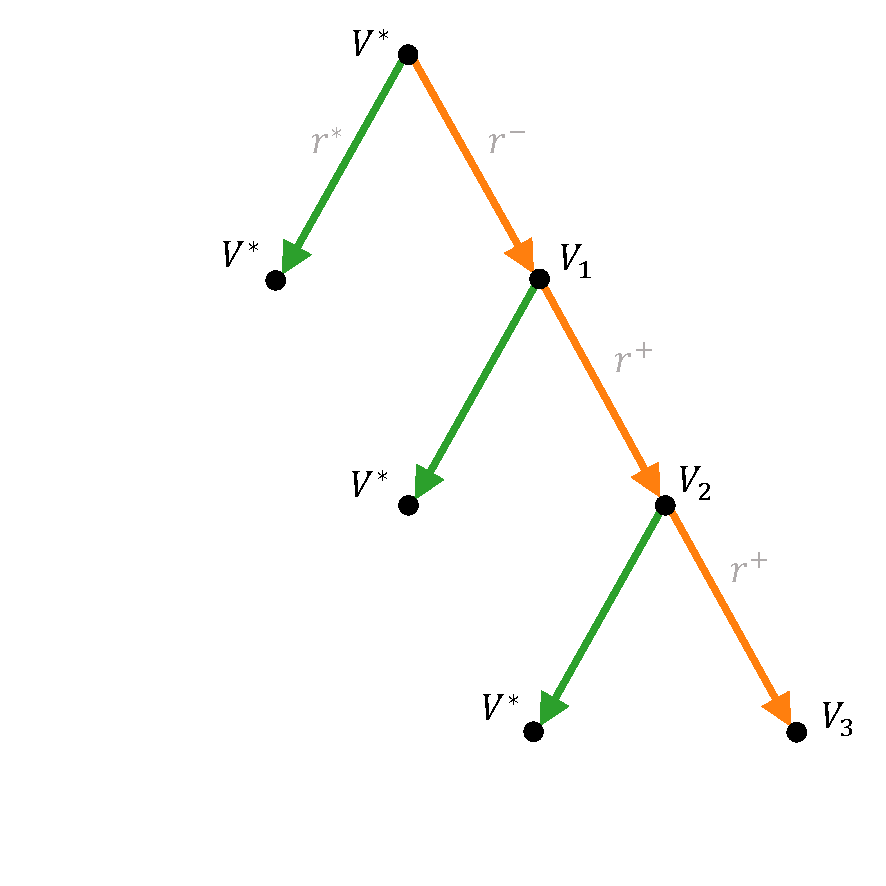
\includegraphics[trim={3.5cm 2cm 0.5cm 0.5cm}, clip, width=0.5\linewidth]{img/mdp_tree.pdf}
    \caption{Planning tree of the MDP $\cM$ of \Cref{fig:mdp}}.
    \label{fig:mdp-tree}
\end{figure}
\begin{lemma}
 Any sequence of actions in $A\setminus{a_1}$ is in $\Tau^\infty$.
\end{lemma}
\begin{proof}
Any such sequence of actions yields the sequence of rewards $r^-, r^+, \dots,r^+$. and end up in the state $s^+$ with value at least $V^\star$ (obtained by further taking $a_1$ indefinitely). Thus its value $V_h$ verifies, 
\begin{align*}
    V_h &\geq \sum_{t=0}^{h-1} \gamma^t r_t + \gamma^h V^\star\\
    &= r^- - r^+ + \sum_{t=0}^{h-1} \gamma^t r^+ + \gamma^h V^\star \\
    &= (-\frac{\gamma}{1-\gamma} - 1)S + \frac{1-\gamma^h}{1-\gamma} (r^\star + S) + \gamma^h V^\star\\
    &= (-\frac{\gamma}{1-\gamma} - 1)S + \frac{1-\gamma^h}{1-\gamma} (r^\star + S) + \gamma^h V^\star\\
    &= V^\star - S\frac{\gamma^h}{1-\gamma} \geq V^\star - \frac{\gamma^h}{1-\gamma}
\end{align*}
\qed\end{proof}

We can directly conclude that $\kappa \geq \limsup{|\{a_2,\dots,a_K\}^h|^{1/h}} = K-1$.

Now, consider the nodes expanded by \Cref{alg:gbop-t}. The first expansion is that of the root, which discovers $s^\star$ and $s^+$. In the absence of information on these two state, the bound $V_{\max}$ is used and the first action $a_1$ gets a higher $\overline{U}$ that any other action $a_2,\dots,a_K$ since $r^\star \geq r^-$. Hence, at the second iteration, the node $a_1$ gets expanded. At this point, the self-loop of the state $s^\star$ is discovered, which means that form now on the bounds verify $L_n(a_1) = V^\star = U_n(a_1)$ for $n\geq2$, which means that $L_n(a_1A^*)-U_n(a_1A^*) = 0$. The nodes $a_2,\dots,a_K$ can be expanded at most once until the entire MDP is discovered and $L_n=V=U_n$ over the entire tree, which means that $\Tau_n^\infty$ is the set of optimal nodes, that is the nodes in the only optimal sequence $a_1^\star$. Hence, $\kappa_\infty = 1.$ 

\section{Efficient Implementation}

\subsection{Update queue}

Instead of executing $\cB_n$ on the entire graph $\cG_n$, we can keep track of the nodes to update in a queue, and propagate these updates to their predecessors.

% TODO: implementation of \cB^$\infty$

\subsection{Early stopping}

$\cB_n^\infty$ can converge in infinite time, as shown in 

\begin{figure}[H]
	\centering
	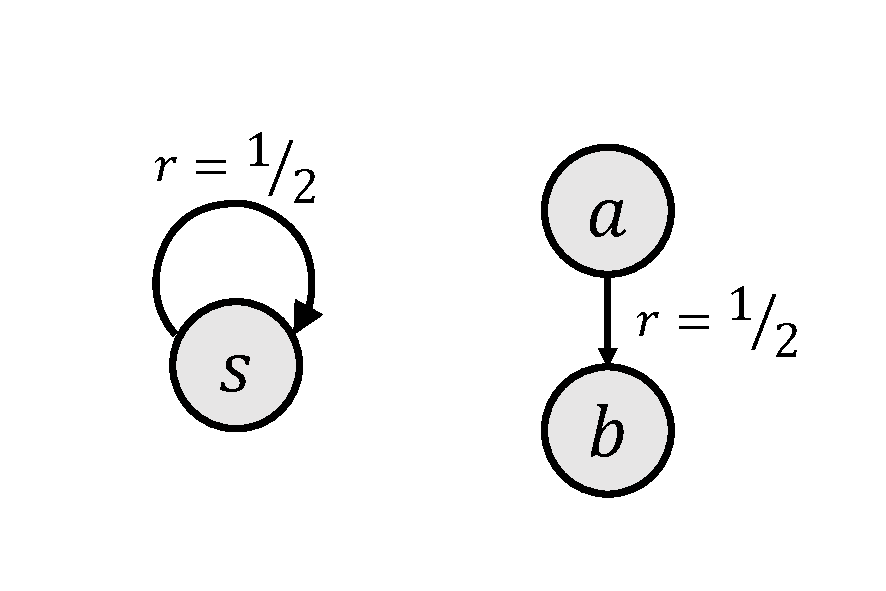
\includegraphics[trim=2.5cm 1cm 1.5cm 2cm, clip, width=0.35\linewidth]{img/loop.pdf}\\
	\begin{tabular}{cccccc}
		\toprule
		Operator & $I$ & $B$ & $M B$ & $\cdots$ & $(M B)^k$ \\
		\midrule
		$U^k(a)$ & $V_{\max}$ & $\frac{1}{2} + \gamma V_{\max}$ & $\frac{1}{2} + \gamma V_{\max}$ && $\frac{1}{2}(1-\gamma^k)V_{\max} + \gamma^k V_{\max}$\\
		$U^k(b)$ & $V_{\max}$ & $V_{\max}$ & $\frac{1}{2} + \gamma V_{\max}$ && $\frac{1}{2}(1-\gamma^k)V_{\max} + \gamma^k V_{\max}$\\
		$L^k(a)$ & $0$ & $\frac{1}{2}$ & $\frac{1}{2}$ && $\frac{1}{2}(1-\gamma^k)V_{\max}$\\
		$L^k(b)$ & $0$ & $0$ & $\frac{1}{2}$ && $\frac{1}{2}(1-\gamma^k)V_{\max}$\\
		\bottomrule
	\end{tabular}
	\caption{\textbf{Top}: a looping MDP with $|S|=|A|=1$, and the corresponding expanded tree $\Tau_1$ after having observed a single transition ($n=1$). \textbf{Bottom}: the sequence of bounds $(U_1^k)$ when alternating $M$ and $B$. $(U_1^k)$ and $(L_1^k)$ converge geometrically to their limit $V = \frac{1}{2}V_{\max}$, thus in infinite time.}
	\label{fig:simple_loop}
\end{figure}


%TODO: prop early stopping here.
Proof of \Cref{prop:early-stopping}
\begin{proof}
	Let $a\in A^h$. We consider the sequence $(\overline{U}_n)_{n\in\Natural}$.
	Notice that for any $U,V\in\Real^\Tau$, we have $\overline{U}(a)-\overline{V}(a)=\gamma^h(U(a)-V(a))$.
	
	Hence, if the premise holds,
	\begin{align*}
	|\overline{U}_{k+1}(a) - \overline{U}_{k}(a)| &\leq \gamma^h\epsilon (1-\gamma)\gamma^{-h-1} = \epsilon (1-\gamma)\gamma^{-1}
	\end{align*}
	
	And then,
	\begin{align*}
	|\overline{U}_{k+1}(a) - \overline{U}_\infty(a)| &= \gamma^h |U_{k+1}(a) - U_\infty(a)|\\
	&\leq \gamma^{h+1}|U_{k}(a) - U_\infty(a)| \text{ since $LA$ is a $\gamma$-contraction}\\
	&\leq \gamma^{h+1}|U_{k}(a) - U_{k+1}(a)| + \gamma^{h+1}|U_{k+1}(a) - U_\infty(a)|\\
	&= \gamma|\overline{U}_{k}(a) - \overline{U}_{k+1}(a)| + \gamma |\overline{U}_{k+1}(a) - \overline{U}_\infty(a)|\\
	&\leq \frac{\gamma}{1-\gamma} |\overline{U}_{k}(a) - \overline{U}_{k+1}(a)|\\
	&\leq\epsilon
	\end{align*}
	\qed\end{proof}


\subsubsection{Experiment on the gridworld domain}

\begin{figure}[H]
	\centering
	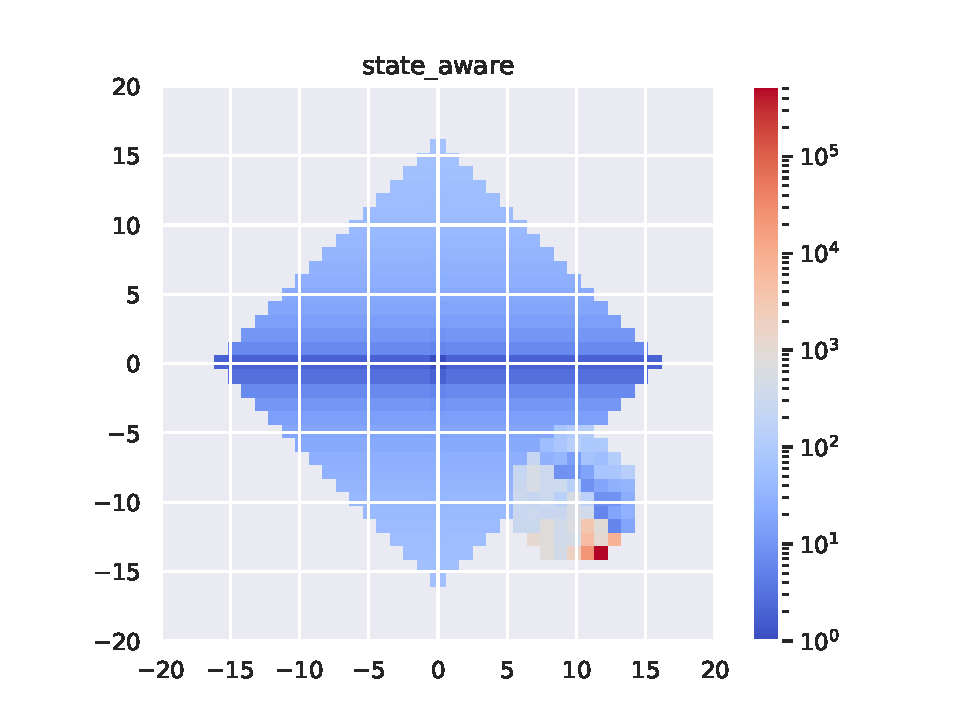
\includegraphics[width=0.44\linewidth]{img/updates_GBOP-D.pdf}
	\caption{Number of updates in the leaf expansion for $n = 5460$, $\gamma=0.95$}
	\label{fig:gw4_updates}
\end{figure}

\begin{figure}[H]
	\centering
	\begin{subfigure}[b]{\linewidth}
		\centering
		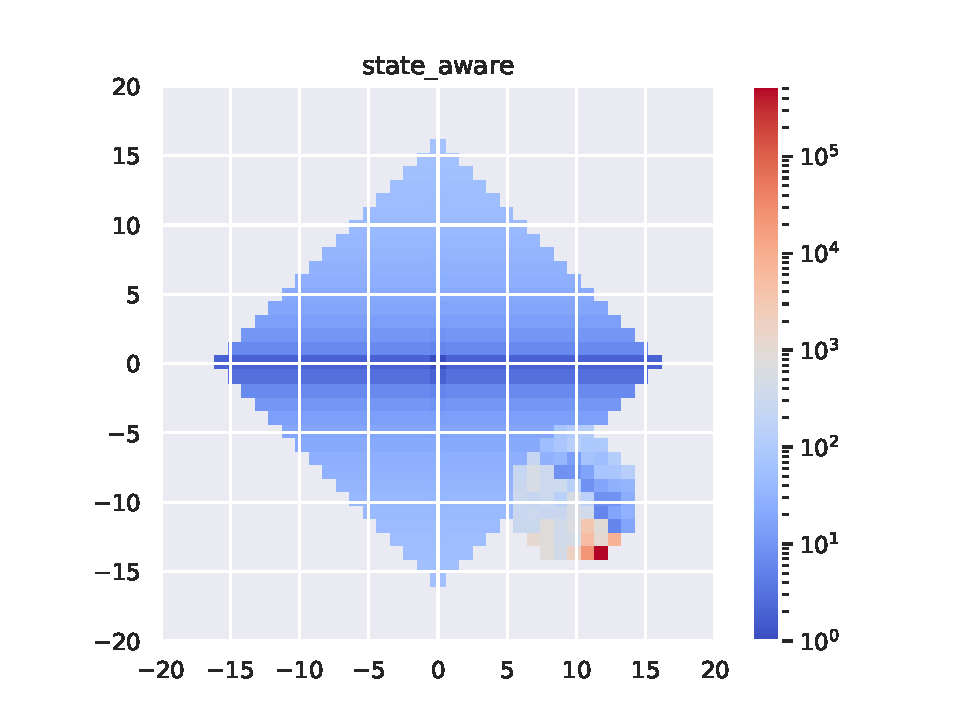
\includegraphics[width=0.49\linewidth]{img/epsilon/0/updates_state_aware.pdf}
		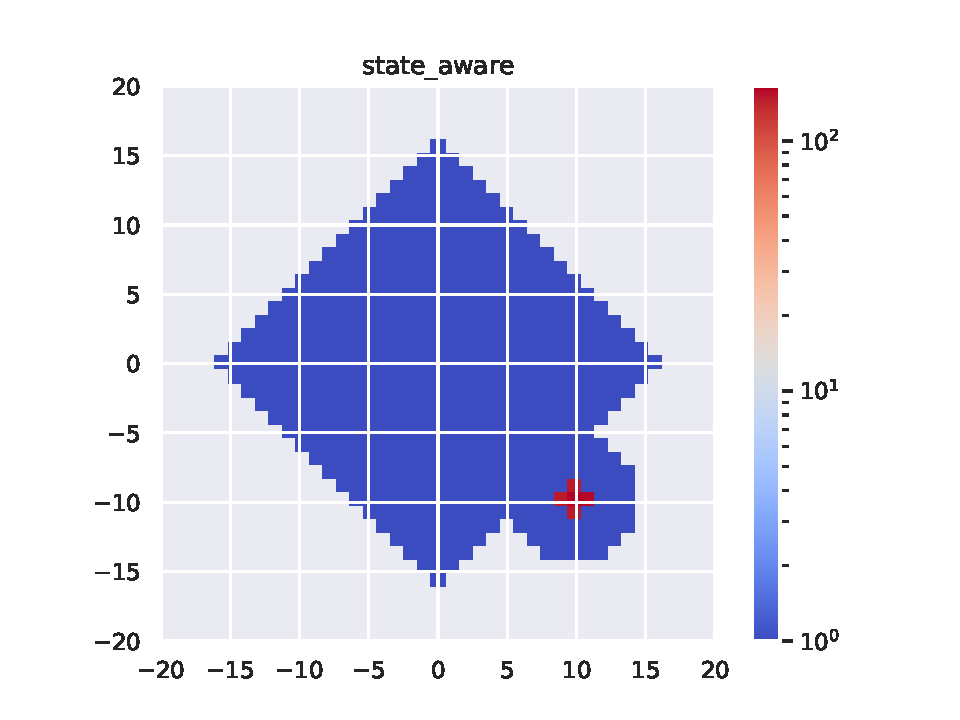
\includegraphics[width=0.49\linewidth]{img/epsilon/0/occupations_state_aware.pdf}
		\caption{$\epsilon=0$}
	\end{subfigure}
	\begin{subfigure}[b]{\linewidth}
		\centering
		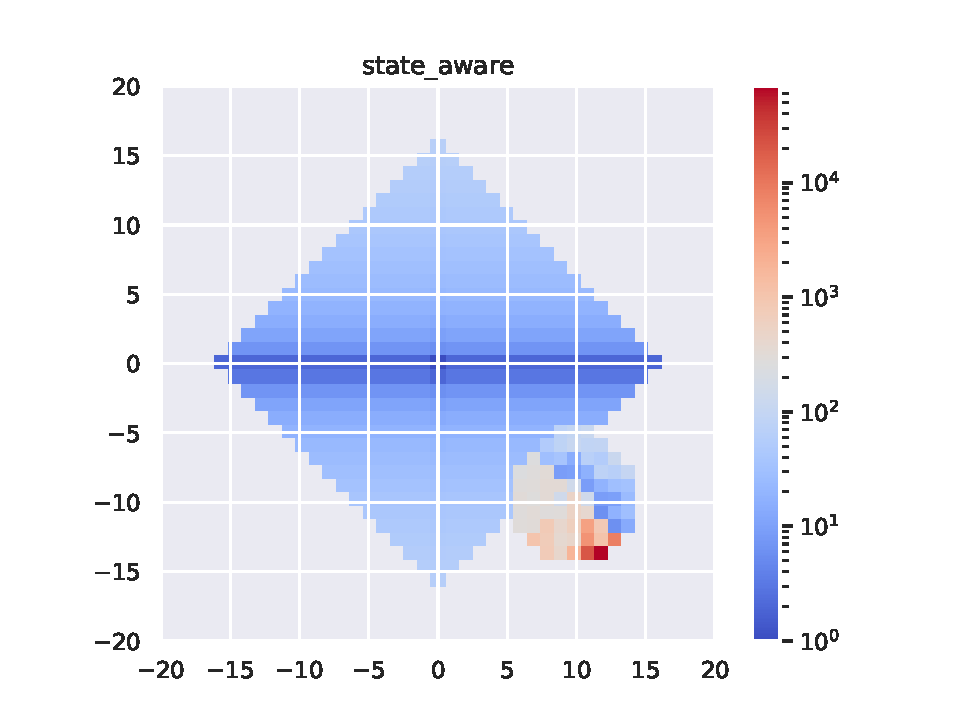
\includegraphics[width=0.49\linewidth]{img/epsilon/1e-2/updates_state_aware.pdf}
		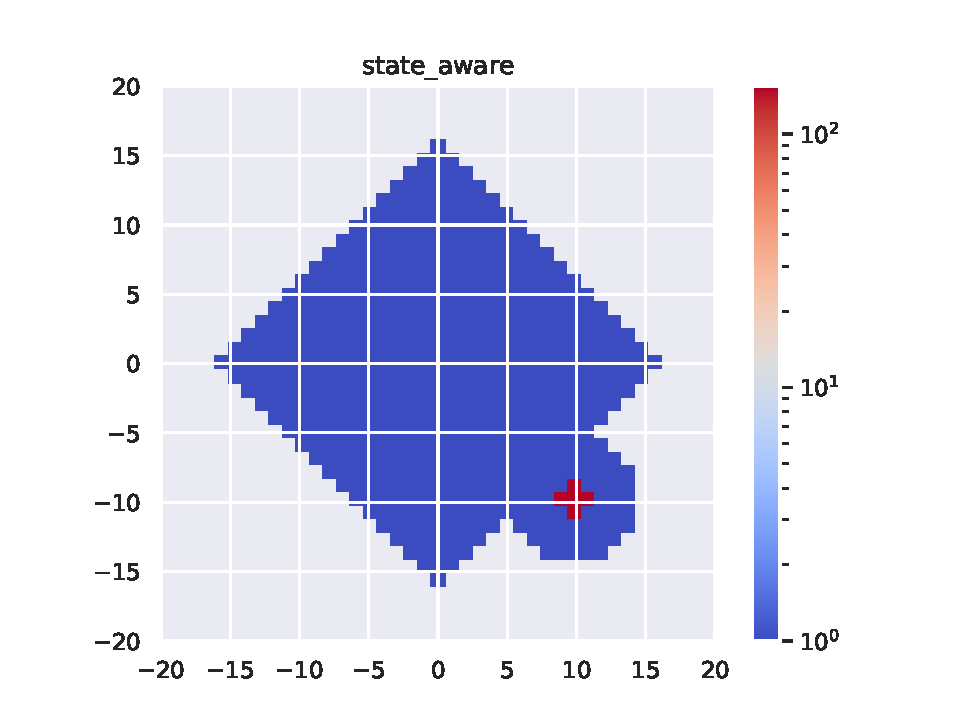
\includegraphics[width=0.49\linewidth]{img/epsilon/1e-2/occupations_state_aware.pdf}
		\caption{$\epsilon=1e-2$}
	\end{subfigure}
	\begin{subfigure}[b]{\linewidth}
		\centering
		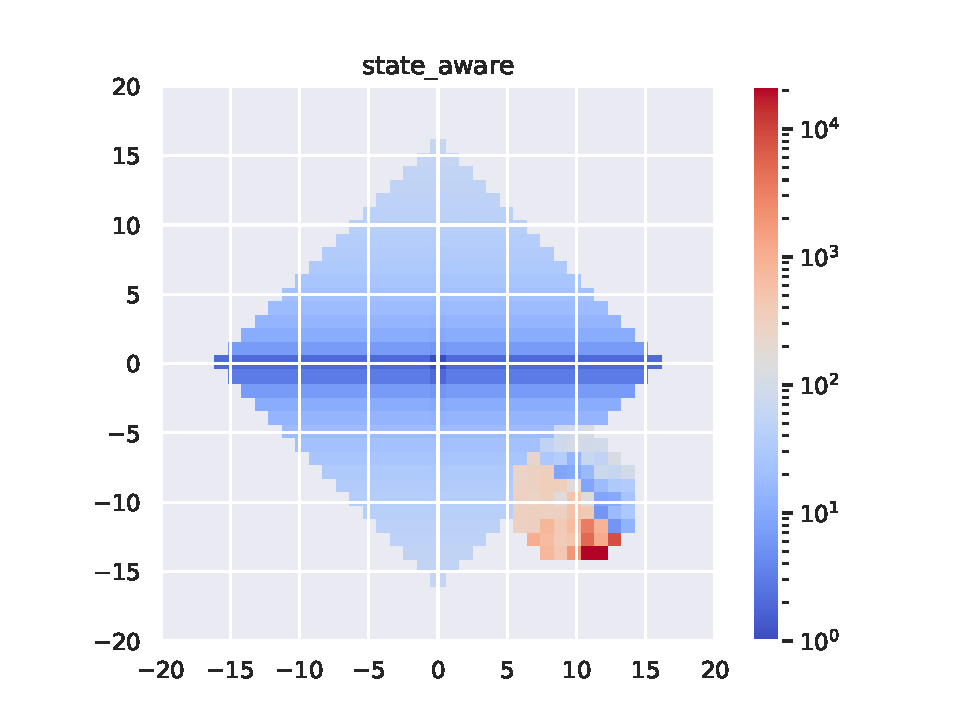
\includegraphics[width=0.49\linewidth]{img/epsilon/1e-1/updates_state_aware.pdf}
		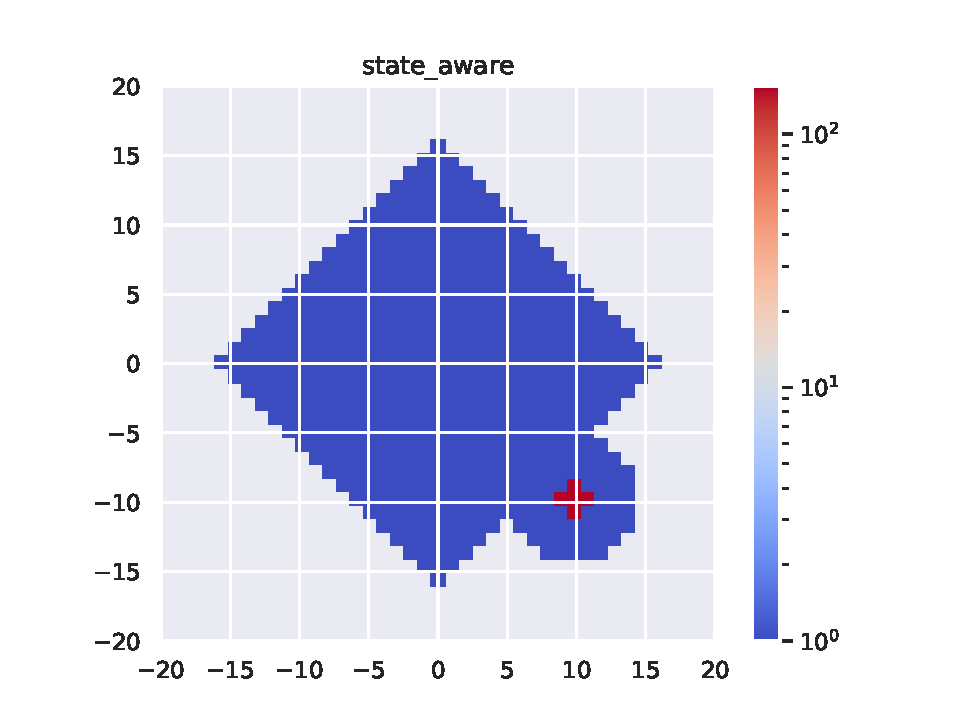
\includegraphics[width=0.49\linewidth]{img/epsilon/1e-2/occupations_state_aware.pdf}
		\caption{$\epsilon=1e-1$}
	\end{subfigure}
	\caption{Updates and occupancies for various values of $\epsilon$, for $n = 5460$, $\gamma=0.95$}
	\label{fig:epsilon_1}
\end{figure}
\begin{figure}[H]
	\ContinuedFloat
	\centering
	\begin{subfigure}[b]{\linewidth}
		\centering
		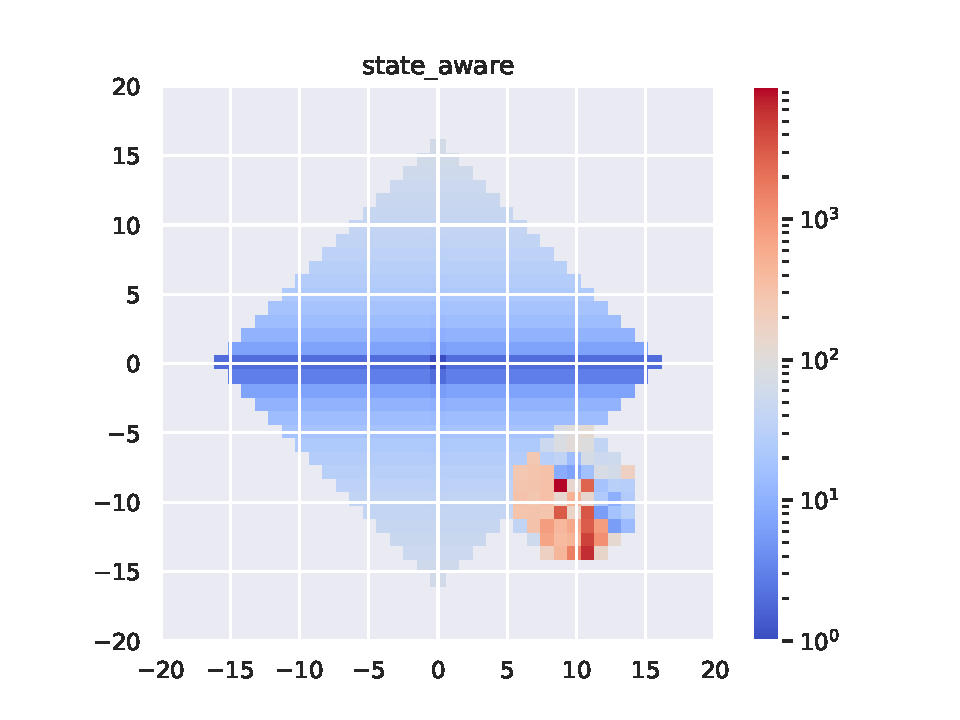
\includegraphics[width=0.49\linewidth]{img/epsilon/1e0/updates_state_aware.pdf}
		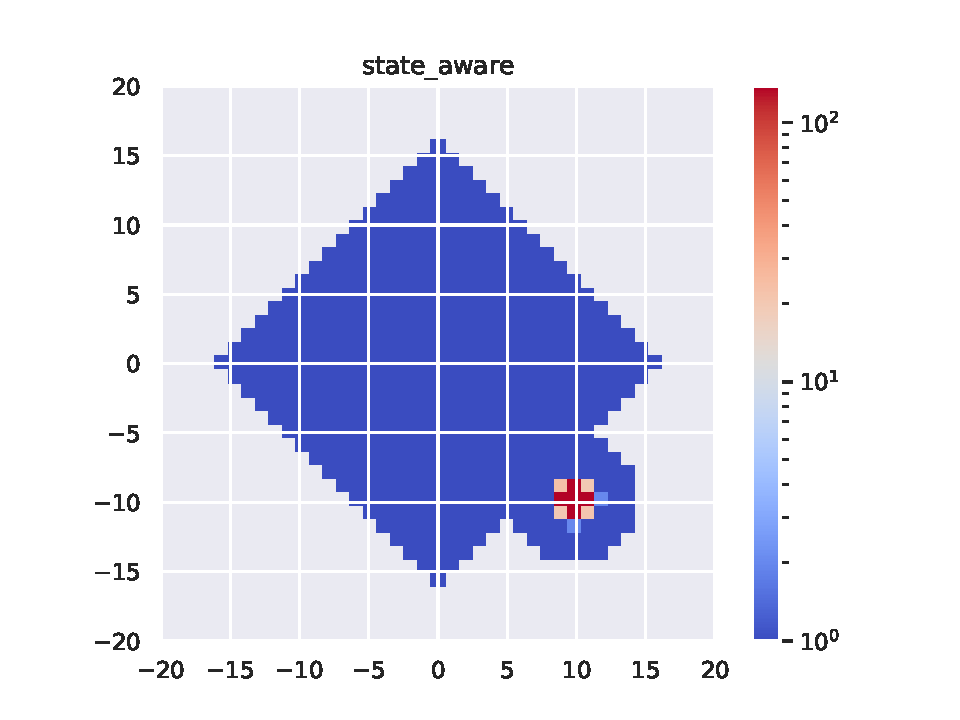
\includegraphics[width=0.49\linewidth]{img/epsilon/1e0/occupations_state_aware.pdf}
		\caption{$\epsilon=1e0$}
	\end{subfigure}
	\begin{subfigure}[b]{\linewidth}
		\centering
		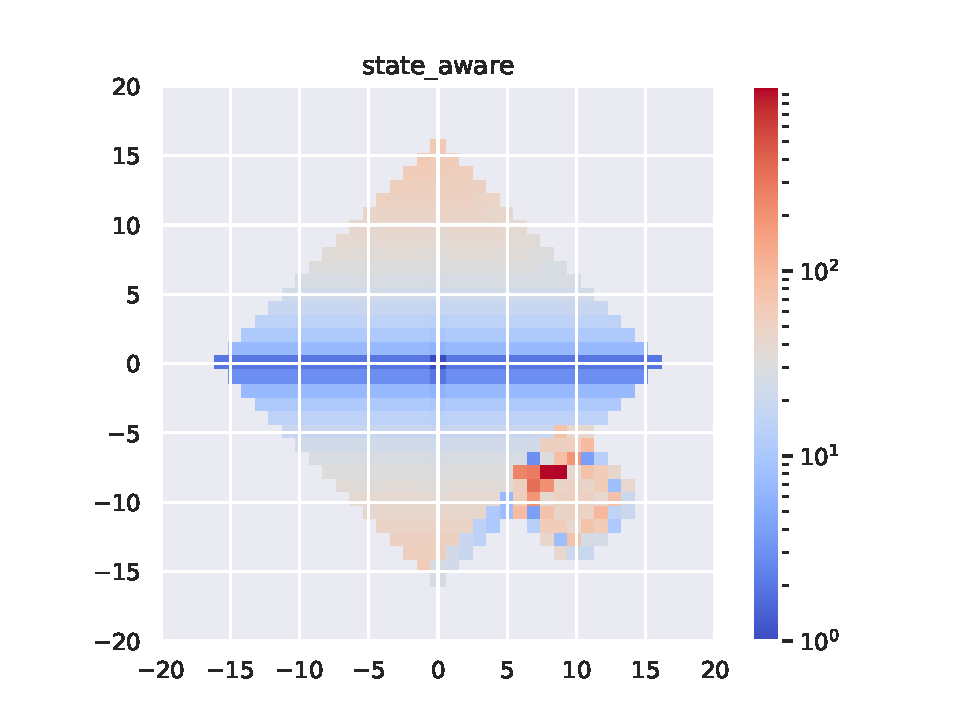
\includegraphics[width=0.49\linewidth]{img/epsilon/1e1/updates_state_aware.pdf}
		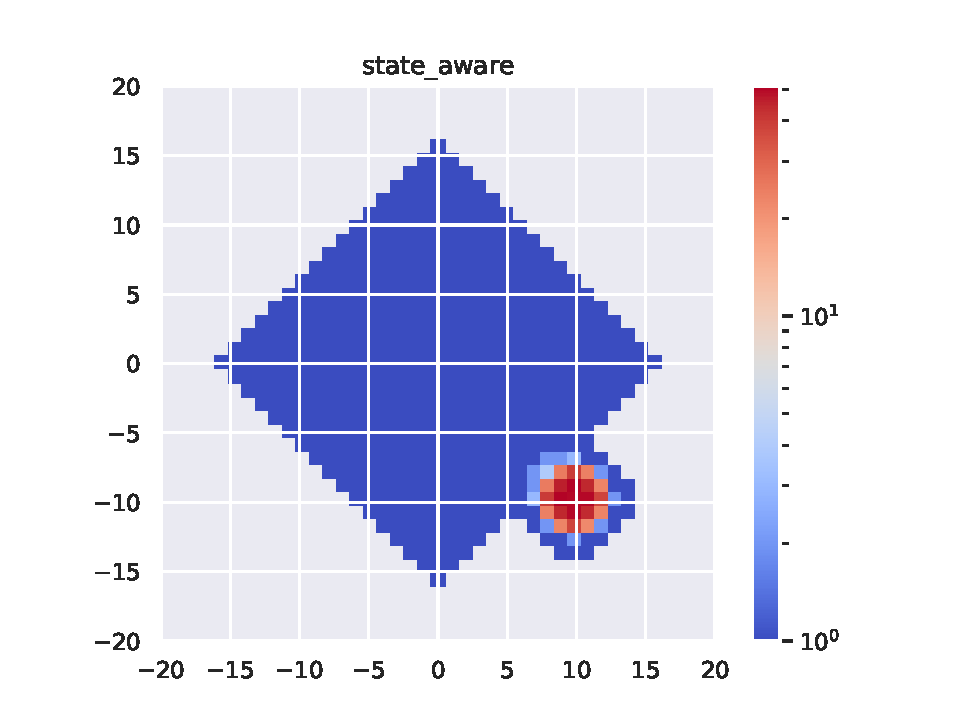
\includegraphics[width=0.49\linewidth]{img/epsilon/1e1/occupations_state_aware.pdf}
		\caption{$\epsilon=1e1$}
	\end{subfigure}
	\begin{subfigure}[b]{\linewidth}
		\centering
		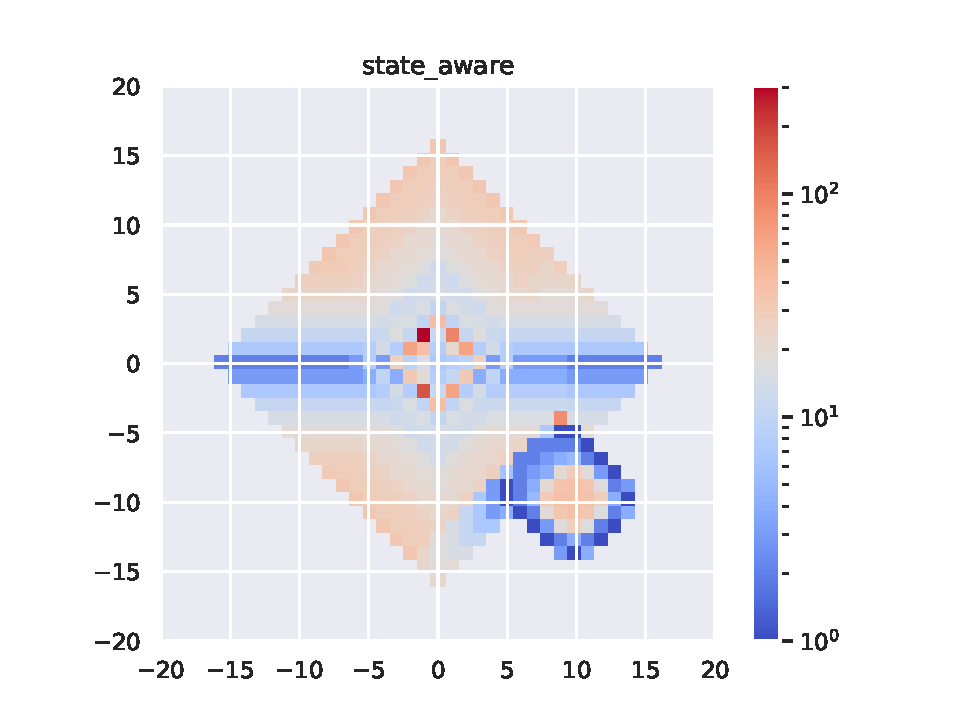
\includegraphics[width=0.49\linewidth]{img/epsilon/1e2/updates_state_aware.pdf}
		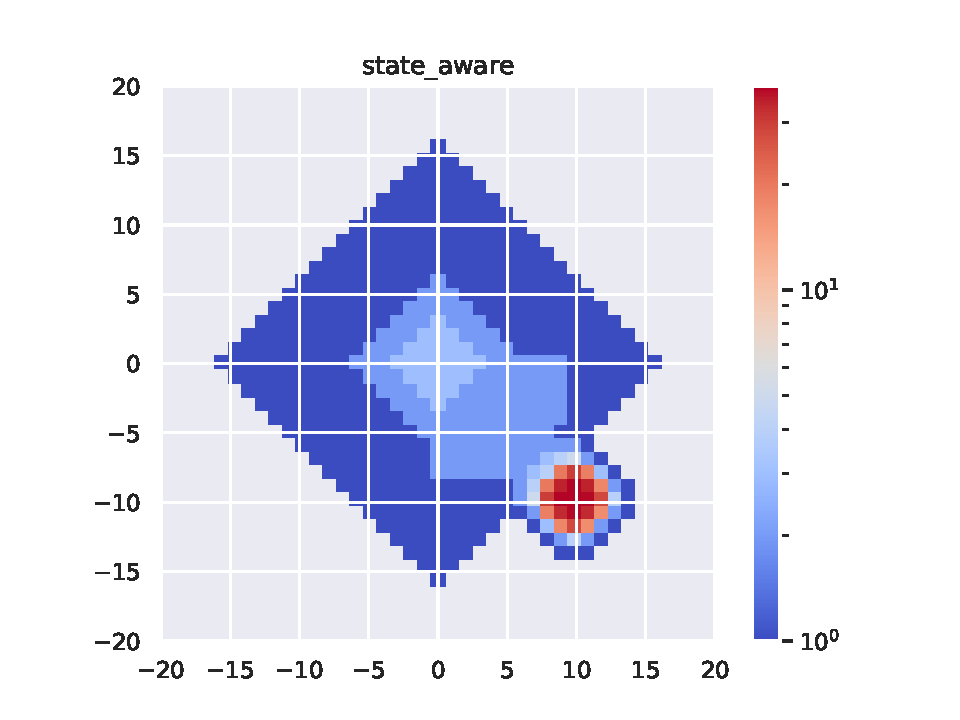
\includegraphics[width=0.49\linewidth]{img/epsilon/1e2/occupations_state_aware.pdf}
		\caption{$\epsilon=1e2 = V_{\max}$}
	\end{subfigure}
	\caption{Updates and occupancies for various values of $\epsilon$, for $n = 5460$, $\gamma=0.95$}
\end{figure}

\section{Supplementary Experiments}

\subsection{State occupancies}

We show the number of times each state is visited by other stochastic planning algorithms, in the stochastic gridworld domain.

\begin{figure}[H]
	\centering
	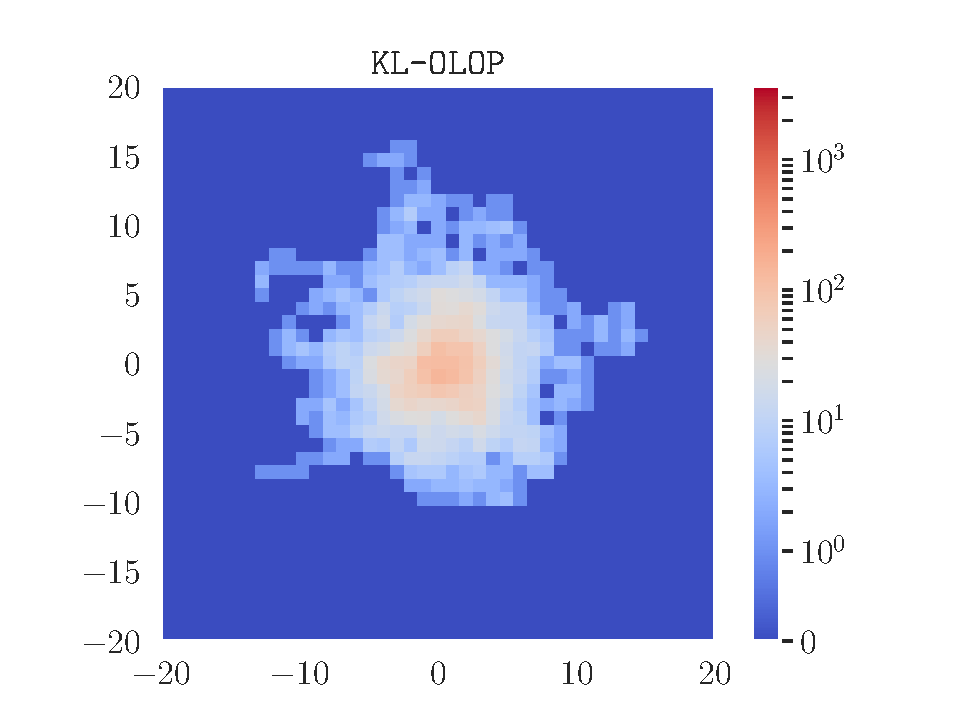
\includegraphics[trim={1.8cm 0.7cm 1.8cm 0.7cm}, clip, width=0.49\linewidth]{img/occupations_KL-OLOP.pdf}
	\hfill
	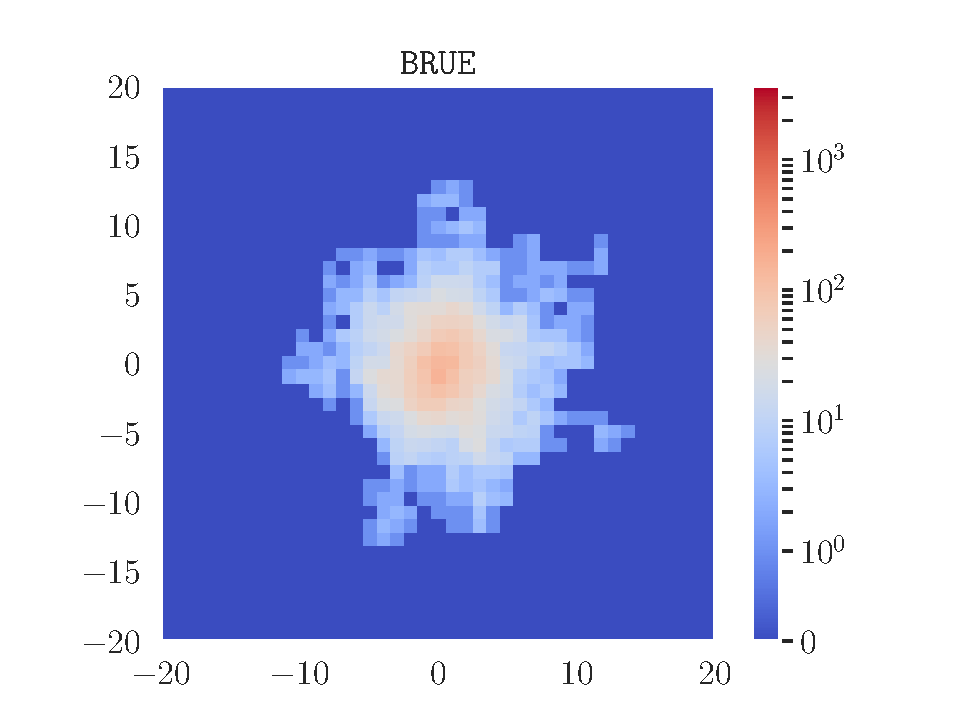
\includegraphics[trim={1.8cm 0.7cm 1.8cm 0.7cm}, clip, width=0.49\linewidth]{img/occupations_BRUE.pdf}
%	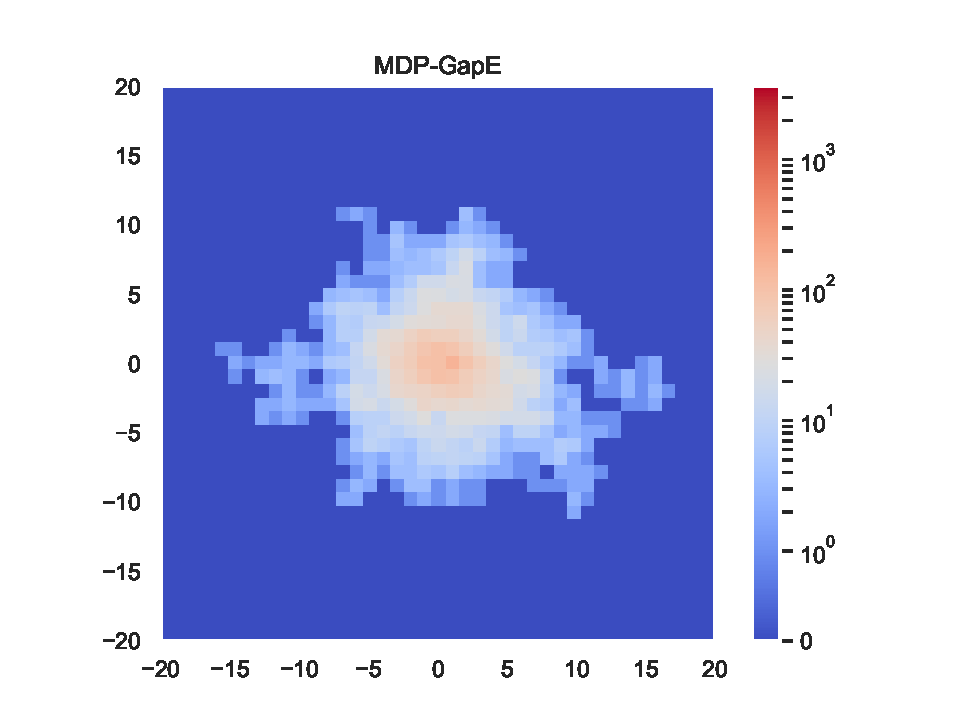
\includegraphics[trim={1.8cm 0.7cm 1.8cm 0.7cm}, clip, width=0.4\linewidth]{img/occupations_MDP-GapE.pdf}
%	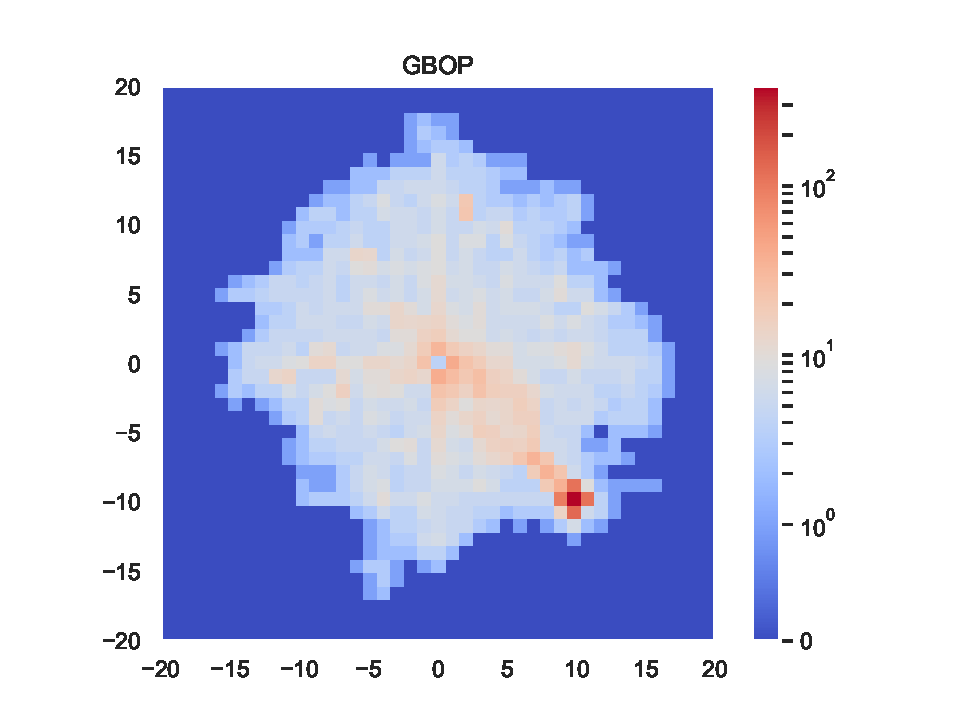
\includegraphics[trim={1.8cm 0.7cm 1.8cm 0.7cm}, clip, width=0.4\linewidth]{img/occupations_GBOP.pdf}
	\caption{State occupancies of other planning algorithms in a stochastic gridworld.}
\end{figure}

\subsection{Expanded trees}
We compare the tree expanded by \OPD and \Cref{alg:gbop-t} in the deterministic gridworld domain. \Cref{fig:trees_expanded} shows that \OPD explored uniformly in the space of sequences, which results in contentrated exploration in the state space as seen in \Cref{fig:deterministic-gridworld}. Conversely, \Cref{alg:gbop-t} expands a sparse unbalanced tree which actually corresponds to uniform exploration in the state space.

\begin{figure}[H]
	\centering
	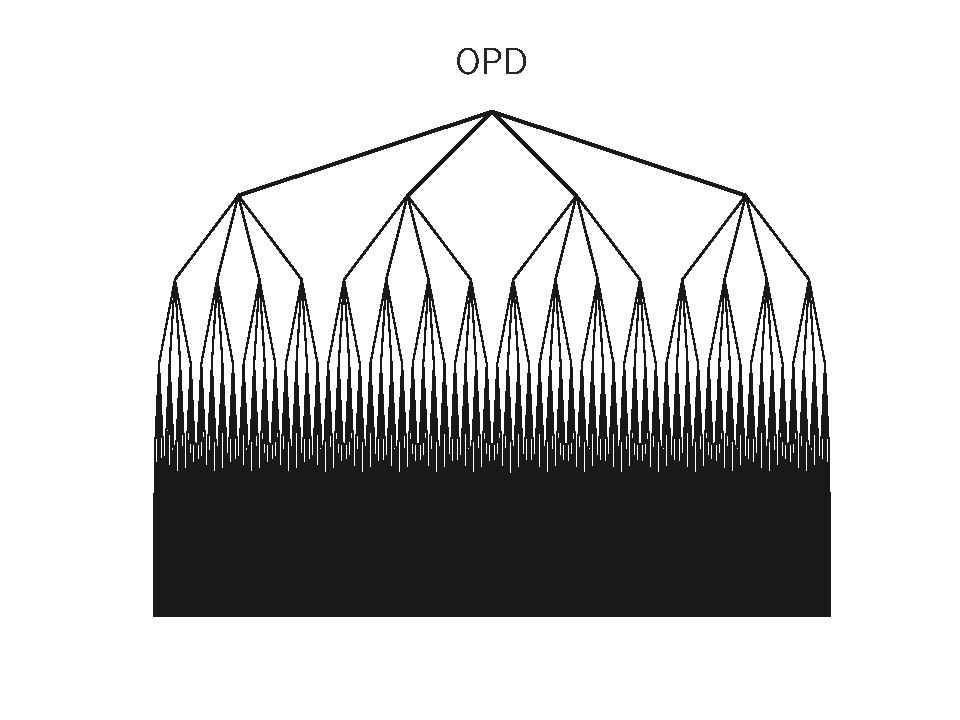
\includegraphics[width=0.44\linewidth]{img/tree_OPD.pdf}
%    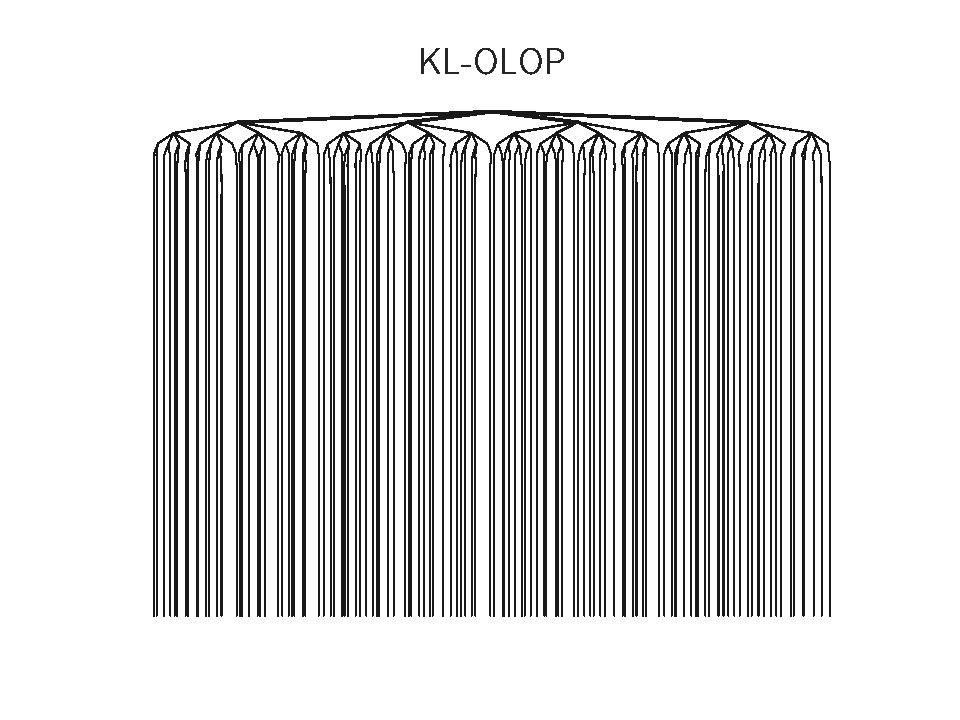
\includegraphics[width=0.44\linewidth]{img/tree_KL-OLOP.pdf}
	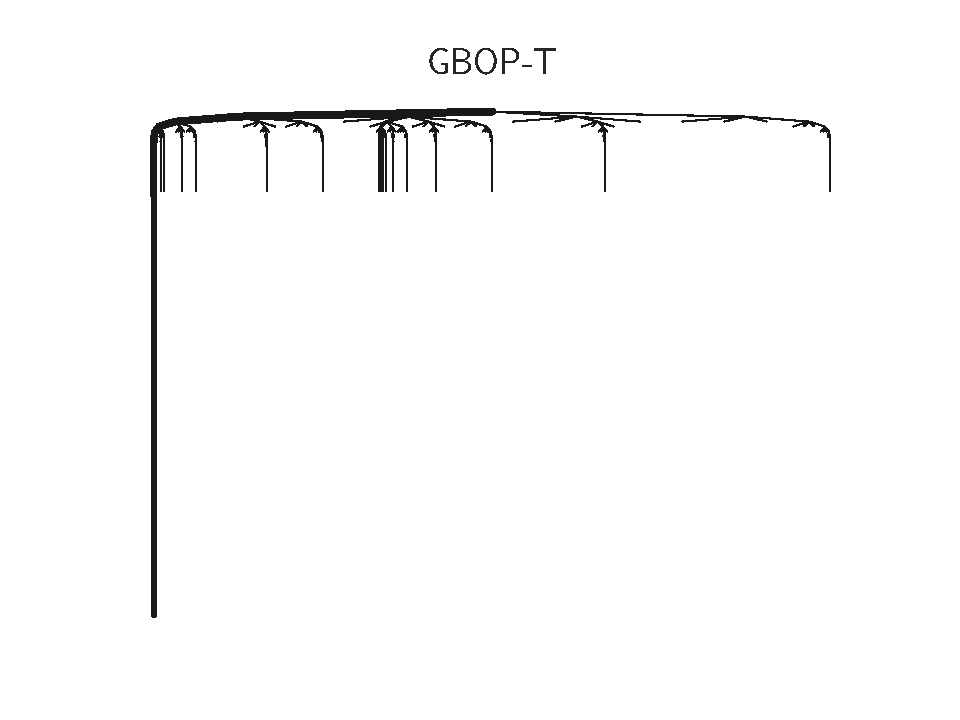
\includegraphics[width=0.44\linewidth]{img/tree_GBOP-T.pdf}
	\caption{Trees expanded for $n = 5460$, $\gamma=0.95$}
	\label{fig:trees_expanded}
\end{figure}

\end{document}
